\documentclass[]{book}
\usepackage{lmodern}
\usepackage{amssymb,amsmath}
\usepackage{ifxetex,ifluatex}
\usepackage{fixltx2e} % provides \textsubscript
\ifnum 0\ifxetex 1\fi\ifluatex 1\fi=0 % if pdftex
  \usepackage[T1]{fontenc}
  \usepackage[utf8]{inputenc}
\else % if luatex or xelatex
  \ifxetex
    \usepackage{mathspec}
  \else
    \usepackage{fontspec}
  \fi
  \defaultfontfeatures{Ligatures=TeX,Scale=MatchLowercase}
\fi
% use upquote if available, for straight quotes in verbatim environments
\IfFileExists{upquote.sty}{\usepackage{upquote}}{}
% use microtype if available
\IfFileExists{microtype.sty}{%
\usepackage{microtype}
\UseMicrotypeSet[protrusion]{basicmath} % disable protrusion for tt fonts
}{}
\usepackage[margin=1in]{geometry}
\usepackage{hyperref}
\hypersetup{unicode=true,
            pdftitle={Datacamp Course on Regression Modeling with Actuarial and Financial Applications},
            pdfauthor={Edward W. (Jed) Frees, University of Wisconsin-Madison},
            pdfborder={0 0 0},
            breaklinks=true}
\urlstyle{same}  % don't use monospace font for urls
\usepackage{natbib}
\bibliographystyle{econPeriod}
\usepackage{color}
\usepackage{fancyvrb}
\newcommand{\VerbBar}{|}
\newcommand{\VERB}{\Verb[commandchars=\\\{\}]}
\DefineVerbatimEnvironment{Highlighting}{Verbatim}{commandchars=\\\{\}}
% Add ',fontsize=\small' for more characters per line
\usepackage{framed}
\definecolor{shadecolor}{RGB}{248,248,248}
\newenvironment{Shaded}{\begin{snugshade}}{\end{snugshade}}
\newcommand{\KeywordTok}[1]{\textcolor[rgb]{0.13,0.29,0.53}{\textbf{#1}}}
\newcommand{\DataTypeTok}[1]{\textcolor[rgb]{0.13,0.29,0.53}{#1}}
\newcommand{\DecValTok}[1]{\textcolor[rgb]{0.00,0.00,0.81}{#1}}
\newcommand{\BaseNTok}[1]{\textcolor[rgb]{0.00,0.00,0.81}{#1}}
\newcommand{\FloatTok}[1]{\textcolor[rgb]{0.00,0.00,0.81}{#1}}
\newcommand{\ConstantTok}[1]{\textcolor[rgb]{0.00,0.00,0.00}{#1}}
\newcommand{\CharTok}[1]{\textcolor[rgb]{0.31,0.60,0.02}{#1}}
\newcommand{\SpecialCharTok}[1]{\textcolor[rgb]{0.00,0.00,0.00}{#1}}
\newcommand{\StringTok}[1]{\textcolor[rgb]{0.31,0.60,0.02}{#1}}
\newcommand{\VerbatimStringTok}[1]{\textcolor[rgb]{0.31,0.60,0.02}{#1}}
\newcommand{\SpecialStringTok}[1]{\textcolor[rgb]{0.31,0.60,0.02}{#1}}
\newcommand{\ImportTok}[1]{#1}
\newcommand{\CommentTok}[1]{\textcolor[rgb]{0.56,0.35,0.01}{\textit{#1}}}
\newcommand{\DocumentationTok}[1]{\textcolor[rgb]{0.56,0.35,0.01}{\textbf{\textit{#1}}}}
\newcommand{\AnnotationTok}[1]{\textcolor[rgb]{0.56,0.35,0.01}{\textbf{\textit{#1}}}}
\newcommand{\CommentVarTok}[1]{\textcolor[rgb]{0.56,0.35,0.01}{\textbf{\textit{#1}}}}
\newcommand{\OtherTok}[1]{\textcolor[rgb]{0.56,0.35,0.01}{#1}}
\newcommand{\FunctionTok}[1]{\textcolor[rgb]{0.00,0.00,0.00}{#1}}
\newcommand{\VariableTok}[1]{\textcolor[rgb]{0.00,0.00,0.00}{#1}}
\newcommand{\ControlFlowTok}[1]{\textcolor[rgb]{0.13,0.29,0.53}{\textbf{#1}}}
\newcommand{\OperatorTok}[1]{\textcolor[rgb]{0.81,0.36,0.00}{\textbf{#1}}}
\newcommand{\BuiltInTok}[1]{#1}
\newcommand{\ExtensionTok}[1]{#1}
\newcommand{\PreprocessorTok}[1]{\textcolor[rgb]{0.56,0.35,0.01}{\textit{#1}}}
\newcommand{\AttributeTok}[1]{\textcolor[rgb]{0.77,0.63,0.00}{#1}}
\newcommand{\RegionMarkerTok}[1]{#1}
\newcommand{\InformationTok}[1]{\textcolor[rgb]{0.56,0.35,0.01}{\textbf{\textit{#1}}}}
\newcommand{\WarningTok}[1]{\textcolor[rgb]{0.56,0.35,0.01}{\textbf{\textit{#1}}}}
\newcommand{\AlertTok}[1]{\textcolor[rgb]{0.94,0.16,0.16}{#1}}
\newcommand{\ErrorTok}[1]{\textcolor[rgb]{0.64,0.00,0.00}{\textbf{#1}}}
\newcommand{\NormalTok}[1]{#1}
\usepackage{longtable,booktabs}
\usepackage{graphicx,grffile}
\makeatletter
\def\maxwidth{\ifdim\Gin@nat@width>\linewidth\linewidth\else\Gin@nat@width\fi}
\def\maxheight{\ifdim\Gin@nat@height>\textheight\textheight\else\Gin@nat@height\fi}
\makeatother
% Scale images if necessary, so that they will not overflow the page
% margins by default, and it is still possible to overwrite the defaults
% using explicit options in \includegraphics[width, height, ...]{}
\setkeys{Gin}{width=\maxwidth,height=\maxheight,keepaspectratio}
\IfFileExists{parskip.sty}{%
\usepackage{parskip}
}{% else
\setlength{\parindent}{0pt}
\setlength{\parskip}{6pt plus 2pt minus 1pt}
}
\setlength{\emergencystretch}{3em}  % prevent overfull lines
\providecommand{\tightlist}{%
  \setlength{\itemsep}{0pt}\setlength{\parskip}{0pt}}
\setcounter{secnumdepth}{5}
% Redefines (sub)paragraphs to behave more like sections
\ifx\paragraph\undefined\else
\let\oldparagraph\paragraph
\renewcommand{\paragraph}[1]{\oldparagraph{#1}\mbox{}}
\fi
\ifx\subparagraph\undefined\else
\let\oldsubparagraph\subparagraph
\renewcommand{\subparagraph}[1]{\oldsubparagraph{#1}\mbox{}}
\fi

%%% Use protect on footnotes to avoid problems with footnotes in titles
\let\rmarkdownfootnote\footnote%
\def\footnote{\protect\rmarkdownfootnote}

%%% Change title format to be more compact
\usepackage{titling}

% Create subtitle command for use in maketitle
\newcommand{\subtitle}[1]{
  \posttitle{
    \begin{center}\large#1\end{center}
    }
}

\setlength{\droptitle}{-2em}
  \title{Datacamp Course on
\texttt{Regression\ Modeling\ with\ Actuarial\ and\ Financial\ Applications}}
  \pretitle{\vspace{\droptitle}\centering\huge}
  \posttitle{\par}
  \author{Edward W. (Jed) Frees, University of Wisconsin-Madison}
  \preauthor{\centering\large\emph}
  \postauthor{\par}
  \date{}
  \predate{}\postdate{}

\usepackage{booktabs}
\setcounter{secnumdepth}{2}

\usepackage{amsthm}
\newtheorem{theorem}{Theorem}[chapter]
\newtheorem{lemma}{Lemma}[chapter]
\theoremstyle{definition}
\newtheorem{definition}{Definition}[chapter]
\newtheorem{corollary}{Corollary}[chapter]
\newtheorem{proposition}{Proposition}[chapter]
\theoremstyle{definition}
\newtheorem{example}{Example}[chapter]
\theoremstyle{definition}
\newtheorem{exercise}{Exercise}[chapter]
\theoremstyle{remark}
\newtheorem*{remark}{Remark}
\newtheorem*{solution}{Solution}
\begin{document}
\maketitle

{
\setcounter{tocdepth}{2}
\tableofcontents
}
\chapter*{Preface}\label{preface}
\addcontentsline{toc}{chapter}{Preface}

\emph{Date: 15 October 2018}

\section*{Acknowledgements}\label{acknowledgements}
\addcontentsline{toc}{section}{Acknowledgements}

Edward Frees acknowledges the John and Anne Oros Distinguished Chair for
Inspired Learning in Business which provided seed money to support the
project. Frees and his Wisconsin colleagues also acknowledge a Society
of Actuaries Center of Excellence Grant that provided funding to support
work in dependence modeling and health initiatives.

We thank Rob Hyndman, Monash University, for allowing us to use his
excellent style files to produce the online version of the book.

We thank Yihui Xie and his colleagues at
\href{https://www.rstudio.com/}{Rstudio} for the
\href{https://bookdown.org/yihui/bookdown/}{R bookdown} package that
allows us to produce this book.

\chapter{Regression and the Normal
Distribution}\label{regression-and-the-normal-distribution}

\textbf{Chapter description}

Regression analysis is a statistical method that is widely used in many
fields of study, with actuarial science being no exception. This chapter
introduces the role of the normal distribution in regression and the use
of logarithmic transformations in specifying regression relationships.

\section{Fitting a normal
distribution}\label{fitting-a-normal-distribution}

In this section, you learn how to:

\begin{itemize}
\tightlist
\item
  Calculate and interpret two basic summary statistics
\item
  Fit a data set to a normal curve
\item
  Calculate probabilities under a standard normal curve
\end{itemize}

\subsection{Video}\label{video}

\subsubsection{Video Overhead}\label{video-overhead}

()

\subsubsection{Video Overhead Details}\label{video-overhead-details}

Show Overhead A. Description of the data details

\hypertarget{toggleOver1.1A}{}
To illustrate a data set that can be analyzed using regression methods,
we consider some data included in Galton's 1885 paper. These data
include the heights of 928 adult children (child\_ht), together with an
index of their parents' height (parent\_ht). Here, all female heights
were multiplied by 1.08, and the index was created by taking the average
of the father's height and rescaled mother's height. Galton was aware
that the parents' and the adult child's height could each be adequately
approximated by a normal curve. In developing regression analysis, he
provided a single model for the joint distribution of heights.

\begin{Shaded}
\begin{Highlighting}[]
\NormalTok{heights <-}\StringTok{ }\KeywordTok{read.csv}\NormalTok{(}\StringTok{"CSVData}\CharTok{\textbackslash{}\textbackslash{}}\StringTok{galton_height.csv"}\NormalTok{,}\DataTypeTok{header =} \OtherTok{TRUE}\NormalTok{)}
\CommentTok{#heights <- read.csv("https://assets.datacamp.com/production/repositories/2610/datasets/c85ede6c205d22049e766bd08956b225c576255b/galton_height.csv", header = TRUE)}
\KeywordTok{plot}\NormalTok{(}\KeywordTok{jitter}\NormalTok{(heights}\OperatorTok{$}\NormalTok{parent_ht),}\KeywordTok{jitter}\NormalTok{(heights}\OperatorTok{$}\NormalTok{child_ht), }\DataTypeTok{ylim =} \KeywordTok{c}\NormalTok{(}\DecValTok{60}\NormalTok{,}\DecValTok{80}\NormalTok{), }\DataTypeTok{xlim =} \KeywordTok{c}\NormalTok{(}\DecValTok{60}\NormalTok{,}\DecValTok{80}\NormalTok{),}
     \DataTypeTok{ylab =} \StringTok{"height of child"}\NormalTok{, }\DataTypeTok{xlab =} \StringTok{"height of parents"}\NormalTok{)}
\KeywordTok{abline}\NormalTok{(}\KeywordTok{lm}\NormalTok{(heights}\OperatorTok{$}\NormalTok{child_ht}\OperatorTok{~}\NormalTok{heights}\OperatorTok{$}\NormalTok{parent_ht))}
\KeywordTok{abline}\NormalTok{(}\DecValTok{0}\NormalTok{,}\DecValTok{1}\NormalTok{,}\DataTypeTok{col =} \StringTok{"red"}\NormalTok{)}
\end{Highlighting}
\end{Shaded}

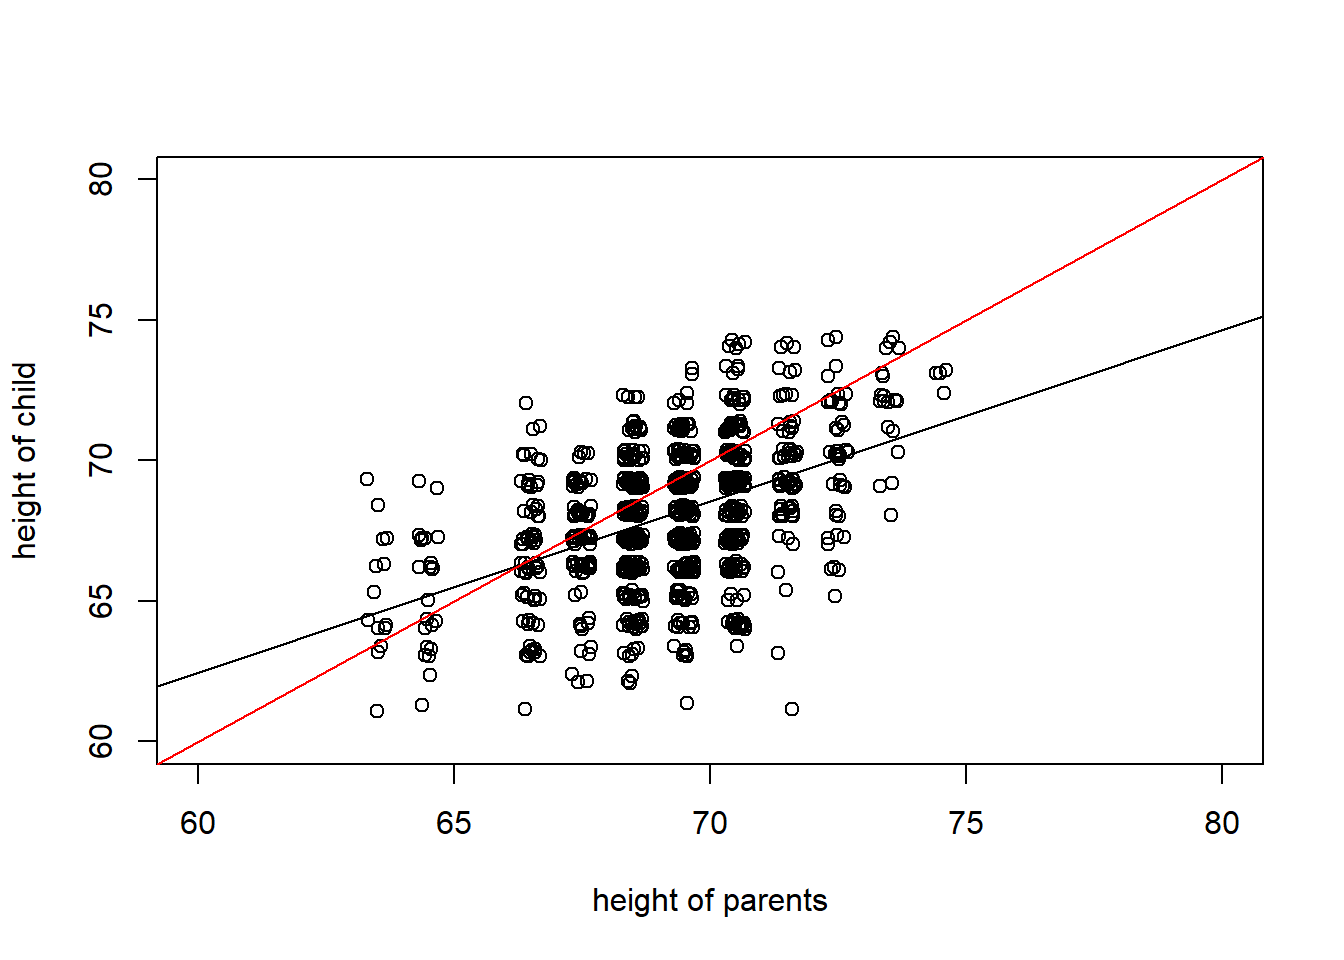
\includegraphics{RegressModelDataCamp_files/figure-latex/unnamed-chunk-2-1.pdf}

Show Overhead B. Read and examine data structure details

\hypertarget{toggleOver1.1B}{}
The data has already been read into a dataset called \texttt{heights}.
Examine the \emph{structure} of the data with the function
\href{https://www.rdocumentation.org/packages/utils/versions/3.5.0/topics/str/}{str()}
and use the
\href{https://www.rdocumentation.org/packages/utils/versions/3.5.0/topics/head/}{head()}
command to looks at the first few records.

\begin{Shaded}
\begin{Highlighting}[]
\NormalTok{heights <-}\StringTok{ }\KeywordTok{read.csv}\NormalTok{(}\StringTok{"CSVData}\CharTok{\textbackslash{}\textbackslash{}}\StringTok{galton_height.csv"}\NormalTok{,}\DataTypeTok{header =} \OtherTok{TRUE}\NormalTok{)}
\CommentTok{#heights <- read.csv("https://assets.datacamp.com/production/repositories/2610/datasets/c85ede6c205d22049e766bd08956b225c576255b/galton_height.csv", header = TRUE)}
\KeywordTok{str}\NormalTok{(heights)}
\KeywordTok{head}\NormalTok{(heights)}
\end{Highlighting}
\end{Shaded}

\begin{verbatim}
'data.frame':   928 obs. of  2 variables:
 $ child_ht : num  72.2 73.2 73.2 73.2 68.2 ...
 $ parent_ht: num  74.5 74.5 74.5 74.5 73.5 73.5 73.5 73.5 73.5 73.5 ...
  child_ht parent_ht
1     72.2      74.5
2     73.2      74.5
3     73.2      74.5
4     73.2      74.5
5     68.2      73.5
6     69.2      73.5
\end{verbatim}

Show Overhead C. Summary stats for parents' height details

\hypertarget{toggleOver1.1C}{}
Next, examine the distribution of the child's height and then examine
the distribution of the parents height.

\begin{Shaded}
\begin{Highlighting}[]
\NormalTok{ht_par <-}\StringTok{ }\NormalTok{heights}\OperatorTok{$}\NormalTok{parent_ht}
\KeywordTok{hist}\NormalTok{(ht_par)}
\end{Highlighting}
\end{Shaded}

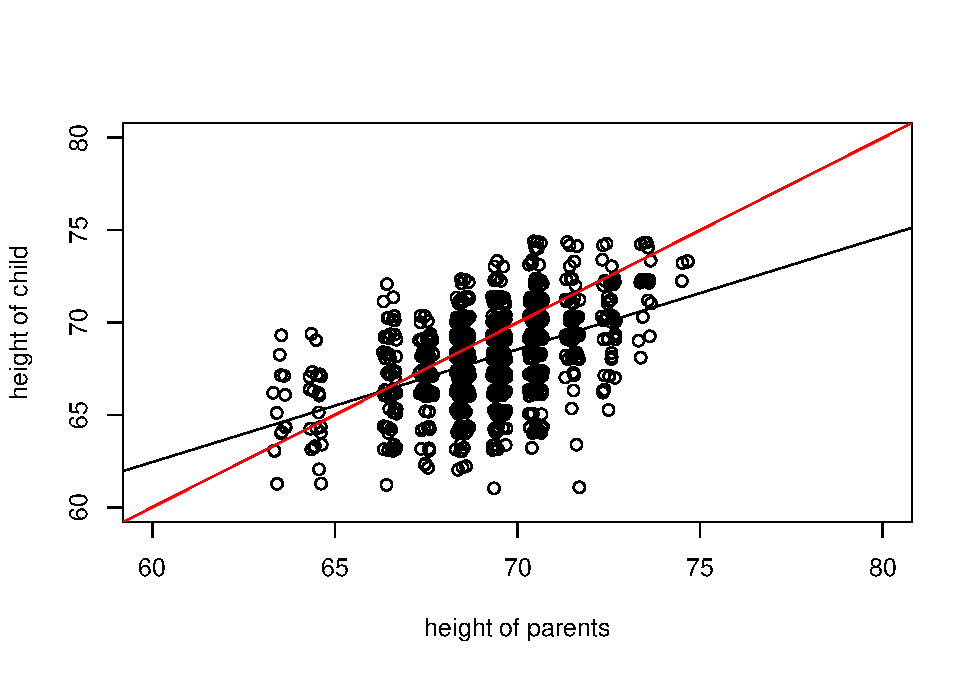
\includegraphics{RegressModelDataCamp_files/figure-latex/unnamed-chunk-4-1.pdf}

\begin{Shaded}
\begin{Highlighting}[]
\KeywordTok{mean}\NormalTok{(ht_par)}
\KeywordTok{sd}\NormalTok{(ht_par)}
\end{Highlighting}
\end{Shaded}

\begin{verbatim}
[1] 69.26293
[1] 1.912274
\end{verbatim}

Show Overhead D. Fit a normal curve to parents' height details

\hypertarget{toggleOver1.1D}{}
\begin{Shaded}
\begin{Highlighting}[]
\NormalTok{(mparent <-}\StringTok{ }\KeywordTok{mean}\NormalTok{(ht_par))}
\NormalTok{(sdparent <-}\StringTok{ }\KeywordTok{sd}\NormalTok{(ht_par))}
\NormalTok{x <-}\StringTok{ }\KeywordTok{seq}\NormalTok{(}\DecValTok{60}\NormalTok{, }\DecValTok{80}\NormalTok{,}\DataTypeTok{by =} \FloatTok{0.1}\NormalTok{)}
\KeywordTok{hist}\NormalTok{(ht_par, }\DataTypeTok{freq =} \OtherTok{FALSE}\NormalTok{)}
\KeywordTok{lines}\NormalTok{(x, }\KeywordTok{dnorm}\NormalTok{(x, }\DataTypeTok{mean =}\NormalTok{ mparent, }\DataTypeTok{sd =}\NormalTok{ sdparent), }\DataTypeTok{col =} \StringTok{"blue"}\NormalTok{)}
\end{Highlighting}
\end{Shaded}

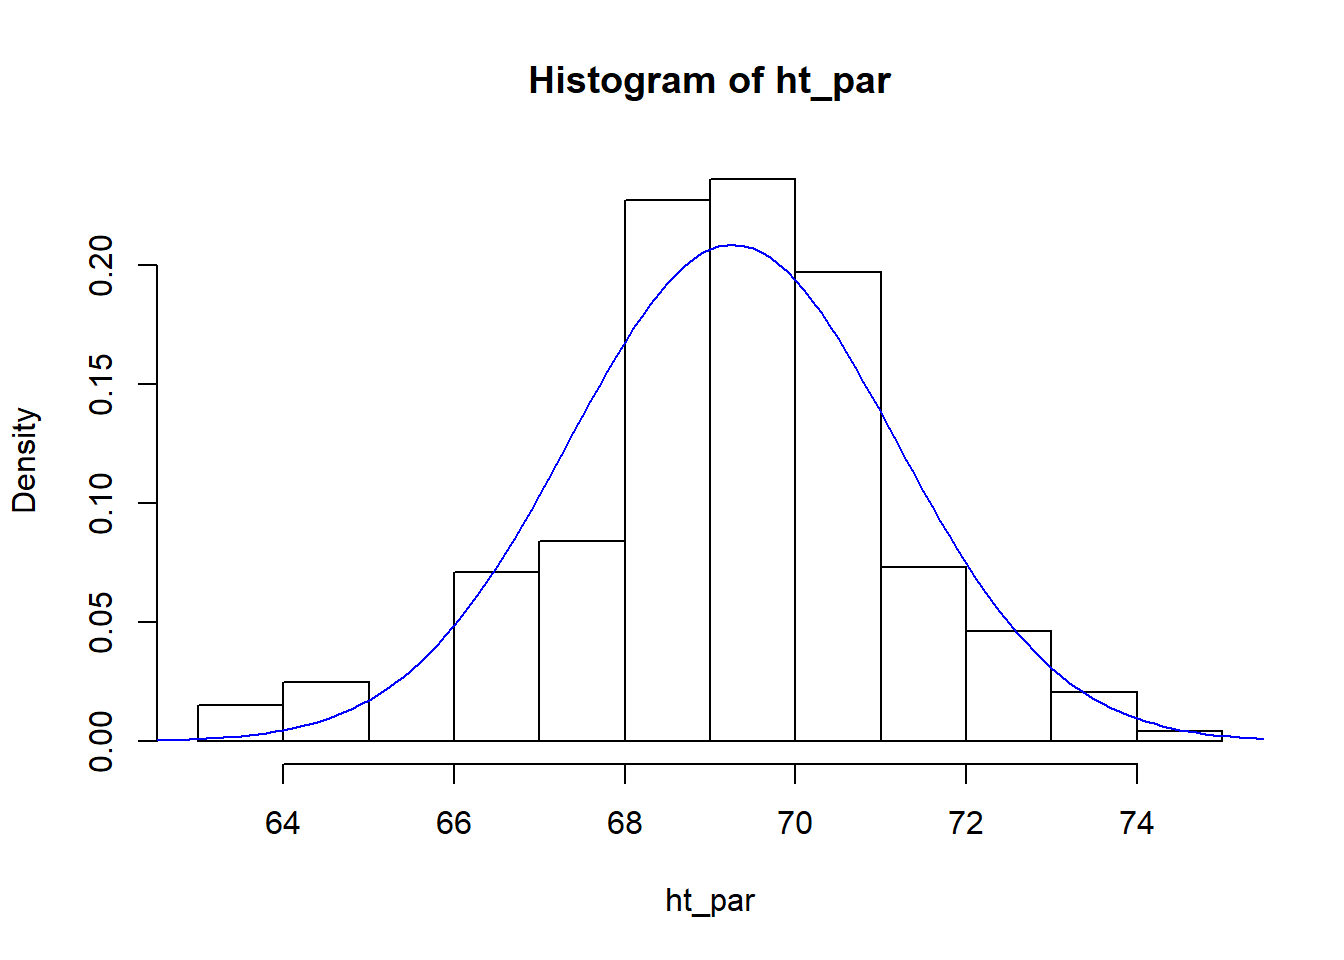
\includegraphics{RegressModelDataCamp_files/figure-latex/unnamed-chunk-5-1.pdf}

\begin{verbatim}
[1] 69.26293
[1] 1.912274
\end{verbatim}

Show Overhead E. Use the normal approximation to determine the
probability of the height of tall parents details

\hypertarget{toggleOver1.1E}{}
\begin{Shaded}
\begin{Highlighting}[]
\NormalTok{TallHeight <-}\StringTok{ }\DecValTok{72}
\KeywordTok{pnorm}\NormalTok{(TallHeight, }\DataTypeTok{mean =}\NormalTok{ mparent, }\DataTypeTok{sd =}\NormalTok{ sdparent)}
\KeywordTok{pnorm}\NormalTok{(}\DecValTok{72}\NormalTok{, }\DataTypeTok{mean =} \KeywordTok{mean}\NormalTok{(ht_par), }\DataTypeTok{sd =} \KeywordTok{sd}\NormalTok{(ht_par))}
\NormalTok{(StdUnitsTallHeight <-}\StringTok{ }\NormalTok{(TallHeight }\OperatorTok{-}\StringTok{ }\NormalTok{mparent)}\OperatorTok{/}\NormalTok{sdparent)}
\KeywordTok{pnorm}\NormalTok{(StdUnitsTallHeight, }\DataTypeTok{mean =} \DecValTok{0}\NormalTok{, }\DataTypeTok{sd =} \DecValTok{1}\NormalTok{)}
\end{Highlighting}
\end{Shaded}

\begin{verbatim}
[1] 0.9238302
[1] 0.9238302
[1] 1.431317
[1] 0.9238302
\end{verbatim}

\subsection{Exercise. Fitting Galton's height
data}\label{exercise.-fitting-galtons-height-data}

\textbf{Assignment Text}

The Galton data has already been read into a dataframe called
\texttt{heights}. These data include the heights of 928 adult children
\texttt{child\_ht}, together with an index of their parents' height
\texttt{parent\_ht}. The video explored the distribution of the parents'
height; in this assignment, we investigate the distribution of the
heights of the adult children.

\textbf{Instructions}

\begin{itemize}
\tightlist
\item
  Define the height of an adult child as a global variable
\item
  Use the function
  \href{https://www.rdocumentation.org/packages/base/versions/3.5.0/topics/mean/}{mean()}
  to calculate the mean and the function
  \href{https://www.rdocumentation.org/packages/base/versions/3.5.0/topics/sd/}{sd()}
  to calculate the standard deviation
\item
  Use the normal approximation and the function
  \href{https://www.rdocumentation.org/packages/stats/versions/3.5.0/topics/Normal/}{pnorm()}
  determine the probability that an adult child's height is less than 72
  inches
\end{itemize}

\textbf{Hint}

Remember that we can reference a variable, say \texttt{var}, from a data
set such as \texttt{heights}, as \texttt{heights\$var}.

eyJsYW5ndWFnZSI6InIiLCJwcmVfZXhlcmNpc2VfY29kZSI6IiMgUHJlLWV4ZXJjaXNlIGNvZGVcbiNoZWlnaHRzIDwtIHJlYWQuY3N2KFwiQ1NWRGF0YVxcXFxnYWx0b25faGVpZ2h0LmNzdlwiLGhlYWRlciA9IFRSVUUpXG5oZWlnaHRzIDwtIHJlYWQuY3N2KFwiaHR0cHM6Ly9hc3NldHMuZGF0YWNhbXAuY29tL3Byb2R1Y3Rpb24vcmVwb3NpdG9yaWVzLzI2MTAvZGF0YXNldHMvYzg1ZWRlNmMyMDVkMjIwNDllNzY2YmQwODk1NmIyMjVjNTc2MjU1Yi9nYWx0b25faGVpZ2h0LmNzdlwiLCBoZWFkZXIgPSBUUlVFKSIsInNhbXBsZSI6IiNEZWZpbmUgdGhlIGdsb2JhbCB2YXJpYWJsZVxuaHRfY2hpbGQgPC0gXG5cbiNDYWxjdWxhdGUgdGhlIG1lYW4gaGVpZ2h0XG4jbWNoaWxkIDwtIFxubWNoaWxkXG5cbiNDYWxjdWxhdGUgdGhlIHN0YW5kYXJkIGRldmlhdGlvbiBvZiBoZWlnaHRzXG4jc2RjaGlsZCA8LSBcbnNkY2hpbGRcblxuI0RldGVybWluZSB0aGUgcHJvYmFiaWxpdHkgdGhhdCB0aGUgaGVpZ2h0IGlzIGxlc3MgdGhhbiA3MlxuX19fKDcyLCBtZWFuPW1jaGlsZCwgc2Q9c2RjaGlsZCkiLCJzb2x1dGlvbiI6IiMgU29sdXRpb25cbmh0X2NoaWxkIDwtIGhlaWdodHMkY2hpbGRfaHRcbm1jaGlsZCA8LSBtZWFuKGh0X2NoaWxkKVxuc2RjaGlsZCA8LSBzZChodF9jaGlsZClcbm1jaGlsZFxuc2RjaGlsZFxucG5vcm0oNzIsIG1lYW4gPSBtY2hpbGQsIHNkID0gc2RjaGlsZCkiLCJzY3QiOiIjIHRlc3RfZXJyb3IoKVxuIyB0ZXN0X29iamVjdChcImh0X2NoaWxkXCIsIGluY29ycmVjdF9tc2cgPSBcIlRoZSBjaGlsZCdzIGhlaWdodCB2YXJpYWJsZSB3YXMgZGVmaW5lZCBpbiB0aGUgd3Jvbmcgd2F5LiAoWW91IG1pZ2h0IGNoZWNrIHRoZSBoaW50LilcIilcbiMgdGVzdF9vYmplY3QoXCJtY2hpbGRcIiwgaW5jb3JyZWN0X21zZyA9IFwiVGhlIG1lYW4gY2hpbGQncyBoZWlnaHQgaXMgY2FsY3VsYXRlZCBpbmNvcnJlY3RseS4gQ2hlY2sgb3V0IHRoZSBtZWFuKCkgZnVuY3Rpb24uXCIpXG4jIHRlc3Rfb2JqZWN0KFwic2RjaGlsZFwiLCBpbmNvcnJlY3RfbXNnID0gXCJUaGUgc3RhbmRhcmQgZGV2aWF0aW9uIG9mIGNoaWxkJ3MgaGVpZ2h0IGlzIGNhbGN1bGF0ZWQgaW5jb3JyZWN0bHkuIENoZWNrIG91dCB0aGUgc2QoKSBmdW5jdGlvbi5cIilcbiN0dXRvcmlhbDo6c3VjY2Vzc19tc2coXCJFeGNlbGxlbnQhIFdpdGggdGhpcyBwcm9jZWR1cmUsIHlvdSBjYW4gbm93IGNhbGN1bGF0ZSBwcm9iYWJpbGl0aWVzIGZvciBhbnkgZGlzdHJpYnV0aW9uIHVzaW5nIGEgbm9ybWFsIGN1cnZlIGFwcHJveGltYXRpb24uXCIpIn0=

\subsection{Exercise. Visualizing child's height
distribution}\label{exercise.-visualizing-childs-height-distribution}

\textbf{Assignment Text}

As in the prior exercise, from the Galton dataset \texttt{heights}, the
heights of 928 adult children have been used to create a global variable
called \texttt{ht\_child}. We also have basic summary statistics, the
mean height \texttt{mchild} and the standard deviation of heights in
\texttt{sdchild}. In this exercise, we explore the fit of the normal
curve to this distribution.

\textbf{Instructions}

\begin{itemize}
\tightlist
\item
  To visualize the distribution, use the function
  \href{https://www.rdocumentation.org/packages/graphics/versions/3.5.0/topics/hist/}{hist()}
  to calculate the histogram. Use the \texttt{freq\ =\ FALSE} option to
  give a histogram with proportions instead of counts.
\item
  Use the function
  \href{https://www.rdocumentation.org/packages/base/versions/3.5.0/topics/seq}{seq()}
  to determine a sequence that can be used for plotting. Then, with the
  function
  \href{https://www.rdocumentation.org/packages/graphics/versions/3.5.0/topics/lines/}{lines()},
  superimpose a normal curve on the histogram
\item
  Determine the probability that a child's height is greater than 72
  inches
\end{itemize}

\textbf{Hint} - Use the function
\href{https://www.rdocumentation.org/packages/stats/versions/3.5.0/topics/Normal/}{dnorm()}
to calculate the normal density, similar to the cumulative probabilites
that you calculated using
\href{https://www.rdocumentation.org/packages/stats/versions/3.5.0/topics/Normal/}{pnorm()}
- To calculate probabilities greater that an amount, simply use 1 minus
the cumulative probability

\textbf{Pre-exercise code}

\begin{Shaded}
\begin{Highlighting}[]
\CommentTok{# Pre-exercise code}
\NormalTok{heights <-}\StringTok{ }\KeywordTok{read.csv}\NormalTok{(}\StringTok{"CSVData}\CharTok{\textbackslash{}\textbackslash{}}\StringTok{galton_height.csv"}\NormalTok{,}\DataTypeTok{header =} \OtherTok{TRUE}\NormalTok{)}
\CommentTok{#heights <- read.csv("https://assets.datacamp.com/production/repositories/2610/datasets/c85ede6c205d22049e766bd08956b225c576255b/galton_height.csv", header = TRUE)}
\NormalTok{ht_child <-}\StringTok{ }\NormalTok{heights}\OperatorTok{$}\NormalTok{child_ht}
\NormalTok{mchild <-}\StringTok{ }\KeywordTok{mean}\NormalTok{(ht_child)}
\NormalTok{sdchild <-}\StringTok{ }\KeywordTok{sd}\NormalTok{(ht_child)}
\end{Highlighting}
\end{Shaded}

\textbf{SampleCode}

\begin{Shaded}
\begin{Highlighting}[]
\StringTok{`}\DataTypeTok{@sample_code}\StringTok{`}
\CommentTok{#Visualize the Distribution}
\KeywordTok{___}\NormalTok{(___, }\DataTypeTok{freq =} \OtherTok{FALSE}\NormalTok{)}

\CommentTok{#Determine a sequence. Then, graph a histogram with a normal curve superimposed}
\NormalTok{x <-}\StringTok{ }\KeywordTok{seq}\NormalTok{(}\DecValTok{60}\NormalTok{, }\DecValTok{80}\NormalTok{,}\DataTypeTok{by =} \FloatTok{0.1}\NormalTok{)}
\KeywordTok{___}\NormalTok{(x, }\KeywordTok{dnorm}\NormalTok{(x,}\DataTypeTok{mean =}\NormalTok{ mchild, }\DataTypeTok{sd =}\NormalTok{ sdchild), }\DataTypeTok{col =} \StringTok{"blue"}\NormalTok{)}

\CommentTok{# Determine the probability that a child's height is greater than 72}
\NormalTok{prob <-}\StringTok{ }\DecValTok{1} \OperatorTok{-}\StringTok{ }
\NormalTok{prob}
\end{Highlighting}
\end{Shaded}

\textbf{Solution}

\begin{Shaded}
\begin{Highlighting}[]
\CommentTok{# Solution}
\KeywordTok{hist}\NormalTok{(ht_child, }\DataTypeTok{freq =} \OtherTok{FALSE}\NormalTok{)}
\NormalTok{x <-}\StringTok{ }\KeywordTok{seq}\NormalTok{(}\DecValTok{60}\NormalTok{, }\DecValTok{80}\NormalTok{,}\DataTypeTok{by =} \FloatTok{0.1}\NormalTok{)}
\KeywordTok{lines}\NormalTok{(x, }\KeywordTok{dnorm}\NormalTok{(x, }\DataTypeTok{mean =}\NormalTok{ mchild, }\DataTypeTok{sd =}\NormalTok{ sdchild), }\DataTypeTok{col =} \StringTok{"blue"}\NormalTok{)}
\end{Highlighting}
\end{Shaded}

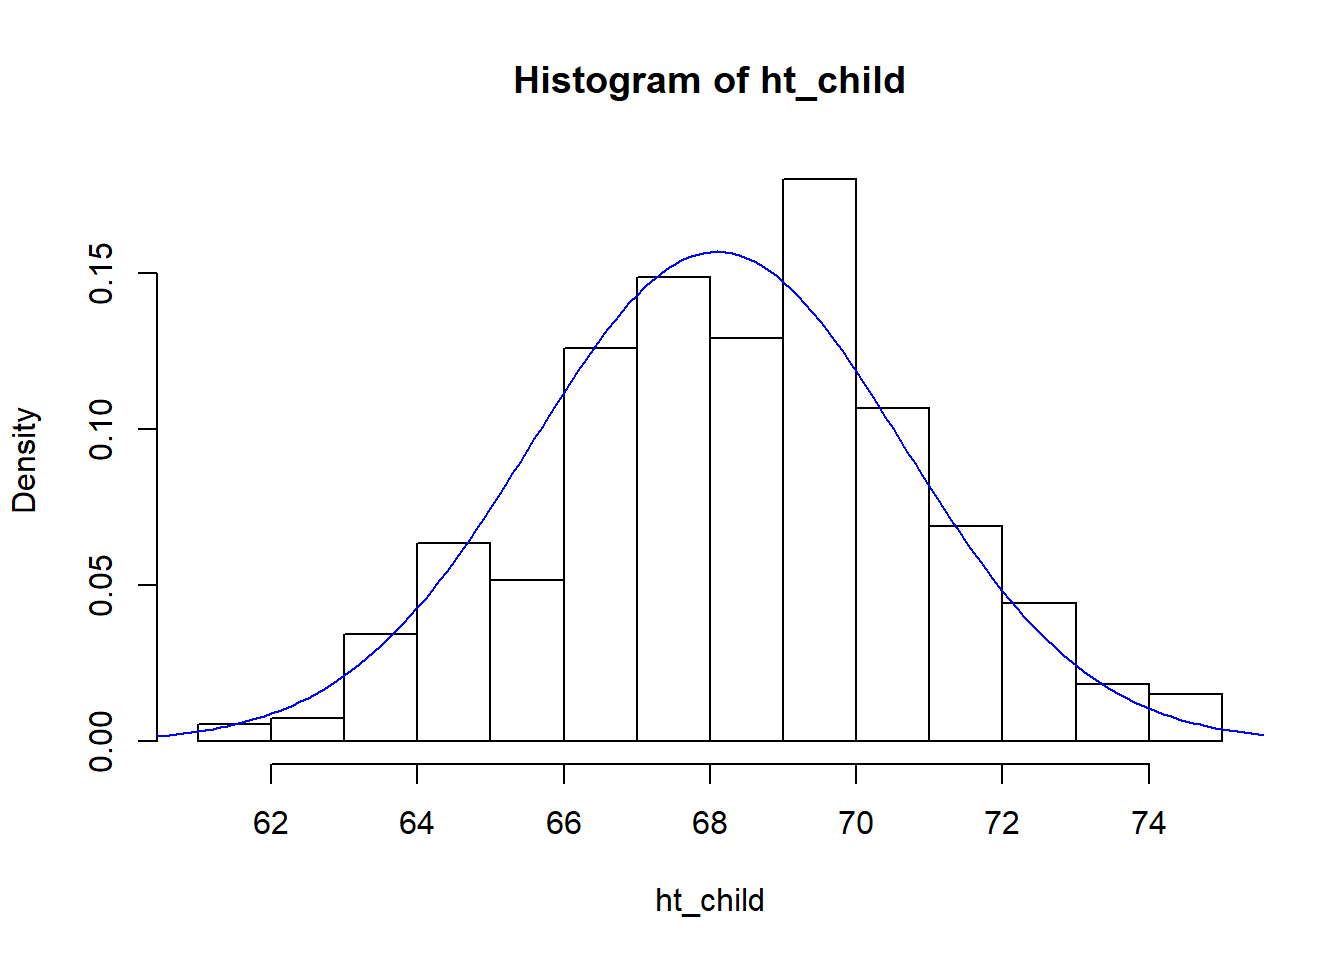
\includegraphics{RegressModelDataCamp_files/figure-latex/unnamed-chunk-14-1.pdf}

\begin{Shaded}
\begin{Highlighting}[]
\NormalTok{prob <-}\StringTok{ }\DecValTok{1} \OperatorTok{-}\StringTok{ }\KeywordTok{pnorm}\NormalTok{(}\DecValTok{72}\NormalTok{, }\DataTypeTok{mean =}\NormalTok{ mchild , }\DataTypeTok{sd =}\NormalTok{ sdchild)}
\NormalTok{prob}
\end{Highlighting}
\end{Shaded}

\begin{verbatim}
[1] 0.0622019
\end{verbatim}

\textbf{Submission Correctness Tests (SCT)} test\_error()
test\_object(``prob'', incorrect\_msg = ``The probability of being
greater than 72 was calculated incorrectly. (You might check the
hint.)'') success\_msg(``Excellent! Visualizing a distribution,
especially with reference to a normal, is important for communicating
results of your analysis.'')

\section{Visualizing distributions}\label{visualizing-distributions}

\subsection{Video (Exercise). Visualizing
distributions}\label{video-exercise.-visualizing-distributions}

\subsubsection{Learning Objectives}\label{learning-objectives}

In this section, you learn how to:

\begin{itemize}
\tightlist
\item
  Calculate and interpret distributions using histograms
\item
  Calculate and interpret distributions using density plots
\end{itemize}

\subsubsection{Video Data Description}\label{video-data-description}

For our first look at an insurance data set, we consider data from
Rempala and Derrig (2005). They considered claims arising from
automobile bodily injury insurance coverages. These are amounts incurred
for outpatient medical treatments that arise from automobile accidents,
typically sprains, broken collarbones and the like. The data consists of
a sample of 272 claims from Massachusetts that were closed in 2001 (by
``closed,'' we mean that the claim is settled and no additional
liabilities can arise from the same accident). Rempala and Derrig were
interested in developing procedures for handling mixtures of ``typical''
claims and others from providers who reported claims fraudulently. For
this sample, we consider only those typical claims, ignoring the
potentially fraudulent ones.

\begin{Shaded}
\begin{Highlighting}[]
\CommentTok{# Reformat Data Set}
\NormalTok{injury <-}\StringTok{ }\KeywordTok{read.csv}\NormalTok{(}\StringTok{"CSVData}\CharTok{\textbackslash{}\textbackslash{}}\StringTok{MassBodilyInjury.csv"}\NormalTok{,}\DataTypeTok{header =} \OtherTok{TRUE}\NormalTok{)}
\KeywordTok{str}\NormalTok{(injury)}
\KeywordTok{head}\NormalTok{(injury)}
\CommentTok{#  PICK THE SUBSET OF THE DATA CORRESPONDING TO PROVIDER A}
\NormalTok{injury2 <-}\StringTok{ }\KeywordTok{subset}\NormalTok{(injury, providerA }\OperatorTok{!}\StringTok{ }\ErrorTok{=}\StringTok{ }\DecValTok{0}\NormalTok{ )}
\NormalTok{injury2}\OperatorTok{$}\NormalTok{claims <-}\StringTok{ }\DecValTok{1000}\OperatorTok{*}\NormalTok{injury2}\OperatorTok{$}\NormalTok{claims}
\NormalTok{injury2}\OperatorTok{$}\NormalTok{logclaims <-}\StringTok{ }\KeywordTok{log}\NormalTok{(injury2}\OperatorTok{$}\NormalTok{claims)}
\NormalTok{injury3 <-}\StringTok{ }\NormalTok{injury2[}\KeywordTok{c}\NormalTok{(}\StringTok{"claims"}\NormalTok{,}\StringTok{"logclaims"}\NormalTok{)]}
\KeywordTok{write.csv}\NormalTok{(injury3,}\StringTok{"CSVData}\CharTok{\textbackslash{}\textbackslash{}}\StringTok{MassBI.csv"}\NormalTok{,}\DataTypeTok{row.names =} \OtherTok{FALSE}\NormalTok{)}
\end{Highlighting}
\end{Shaded}

\subsubsection{Video}\label{video-1}

\textbf{Overhead A. Bring in Data, Introduce Logarithmic Claims}

\begin{Shaded}
\begin{Highlighting}[]
\NormalTok{injury <-}\StringTok{ }\KeywordTok{read.csv}\NormalTok{(}\StringTok{"CSVData}\CharTok{\textbackslash{}\textbackslash{}}\StringTok{MassBI.csv"}\NormalTok{,}\DataTypeTok{header =} \OtherTok{TRUE}\NormalTok{)}
\CommentTok{#  CHECK THE NAMES, DIMENSION IN THE FILE AND LIST THE FIRST 8 OBSERVATIONS  ;}
\KeywordTok{str}\NormalTok{(injury)}
\KeywordTok{head}\NormalTok{(injury)}
\KeywordTok{attach}\NormalTok{(injury)}
\NormalTok{claims <-}\StringTok{ }\NormalTok{injury}\OperatorTok{$}\NormalTok{claims}
\KeywordTok{par}\NormalTok{(}\DataTypeTok{mfrow =} \KeywordTok{c}\NormalTok{(}\DecValTok{1}\NormalTok{, }\DecValTok{2}\NormalTok{))}
\KeywordTok{hist}\NormalTok{(claims)}
\KeywordTok{hist}\NormalTok{(logclaims)}
\end{Highlighting}
\end{Shaded}

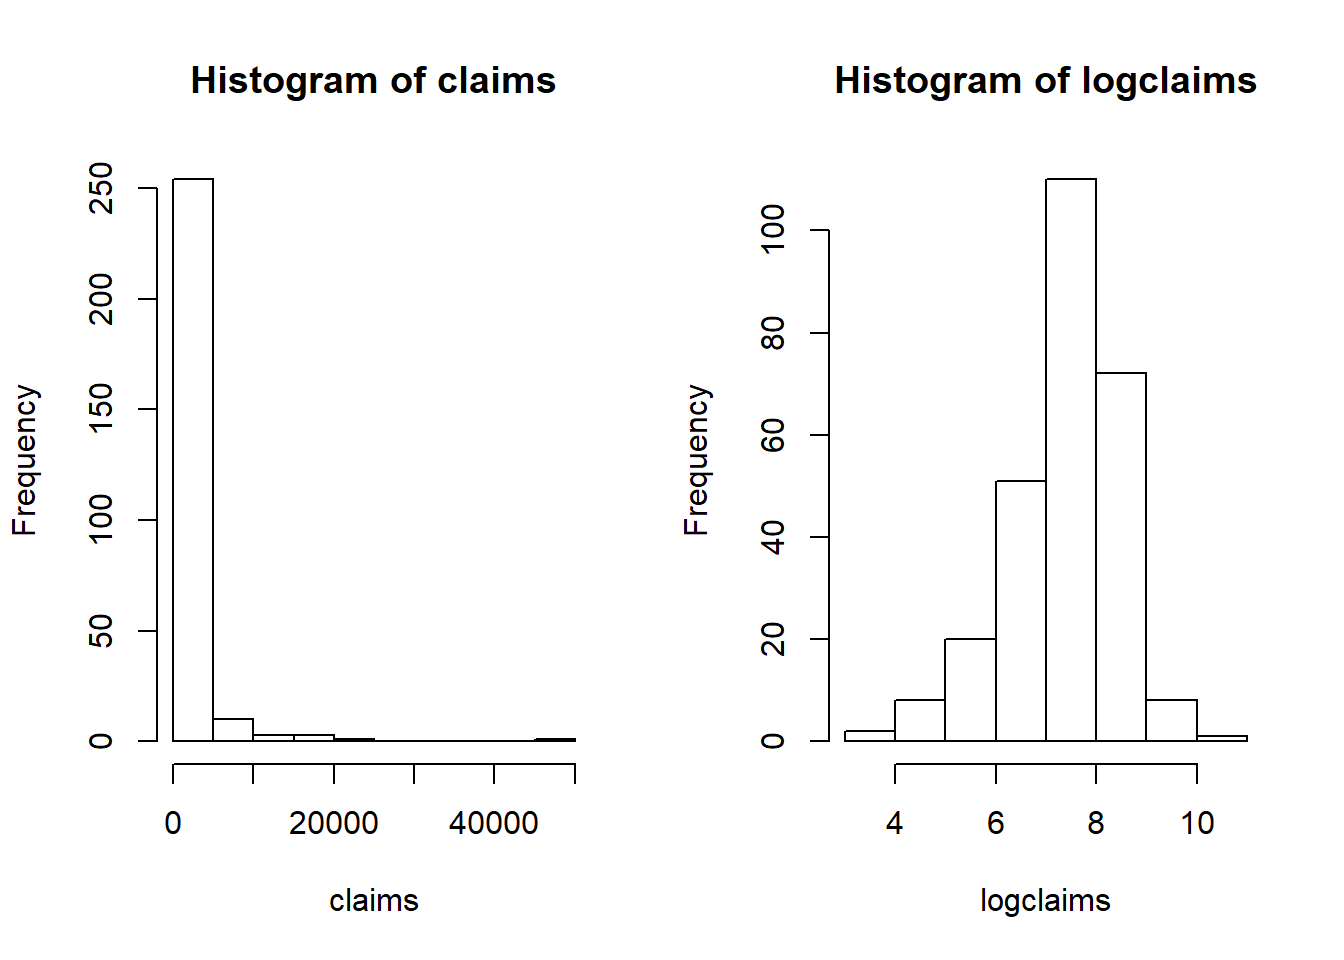
\includegraphics{RegressModelDataCamp_files/figure-latex/unnamed-chunk-16-1.pdf}

\begin{verbatim}
'data.frame':   272 obs. of  2 variables:
 $ claims   : int  45 47 70 75 77 92 117 117 140 145 ...
 $ logclaims: num  3.81 3.85 4.25 4.32 4.34 ...
  claims logclaims
1     45  3.806662
2     47  3.850148
3     70  4.248495
4     75  4.317488
5     77  4.343805
6     92  4.521789
\end{verbatim}

\textbf{Overhead B. Show how to get a finer grid for histograms}

\begin{Shaded}
\begin{Highlighting}[]
\KeywordTok{par}\NormalTok{(}\DataTypeTok{mfrow =} \KeywordTok{c}\NormalTok{(}\DecValTok{1}\NormalTok{, }\DecValTok{2}\NormalTok{))}
\KeywordTok{hist}\NormalTok{(logclaims)}
\KeywordTok{hist}\NormalTok{(logclaims,}\DataTypeTok{breaks =} \DecValTok{15}\NormalTok{)}
\end{Highlighting}
\end{Shaded}

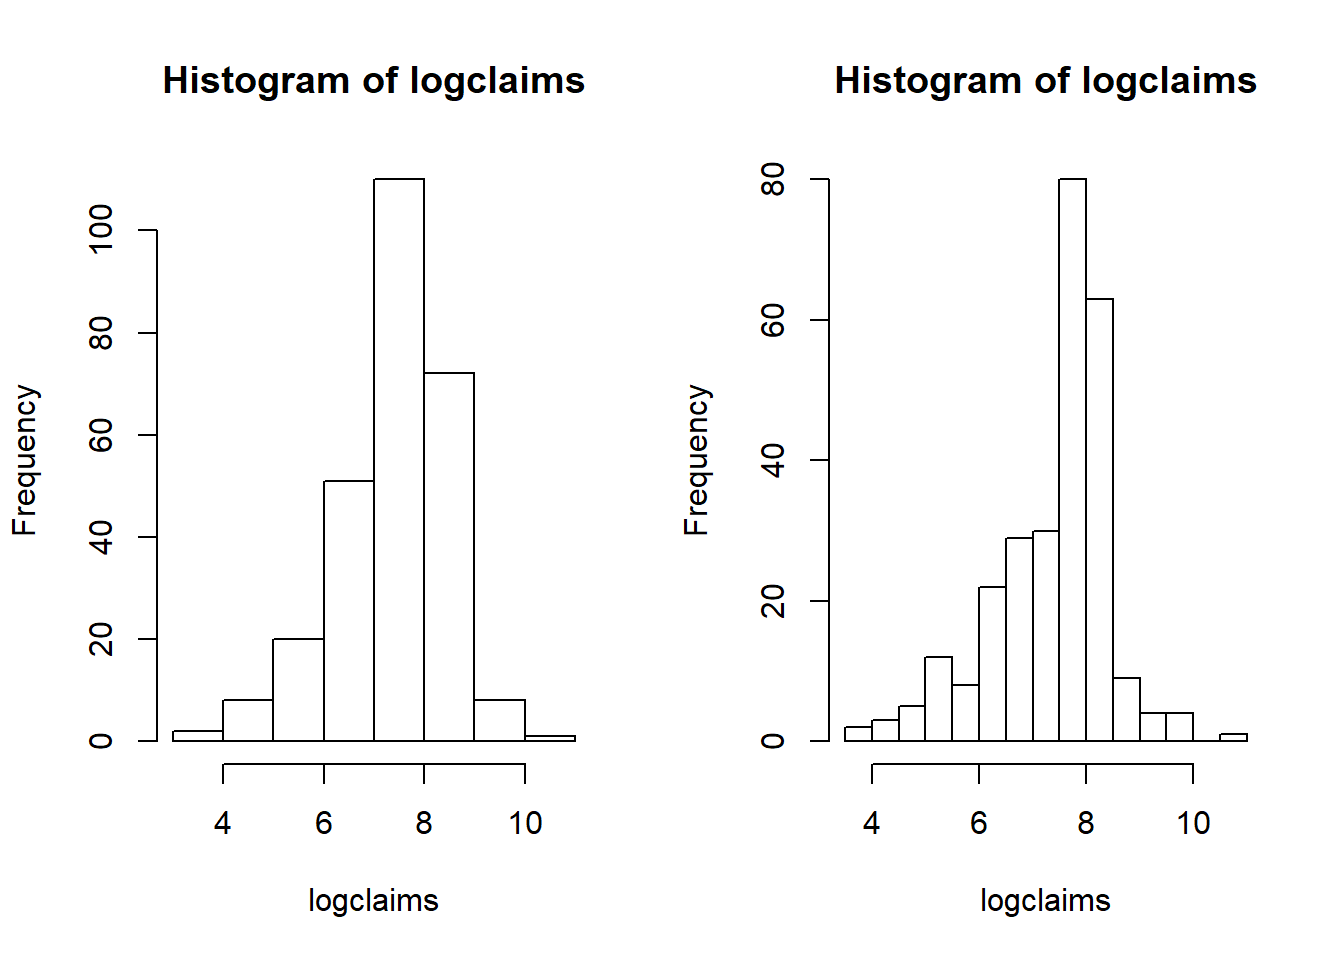
\includegraphics{RegressModelDataCamp_files/figure-latex/unnamed-chunk-17-1.pdf}

\textbf{Overhead C. Introduce the density plot}

\begin{Shaded}
\begin{Highlighting}[]
\KeywordTok{par}\NormalTok{(}\DataTypeTok{mfrow =} \KeywordTok{c}\NormalTok{(}\DecValTok{1}\NormalTok{, }\DecValTok{2}\NormalTok{))}
\KeywordTok{plot}\NormalTok{(}\KeywordTok{density}\NormalTok{(logclaims))}
\KeywordTok{hist}\NormalTok{(logclaims, }\DataTypeTok{breaks =} \DecValTok{15}\NormalTok{,}\DataTypeTok{freq =} \OtherTok{FALSE}\NormalTok{)}
\KeywordTok{lines}\NormalTok{(}\KeywordTok{density}\NormalTok{(logclaims))}
\end{Highlighting}
\end{Shaded}

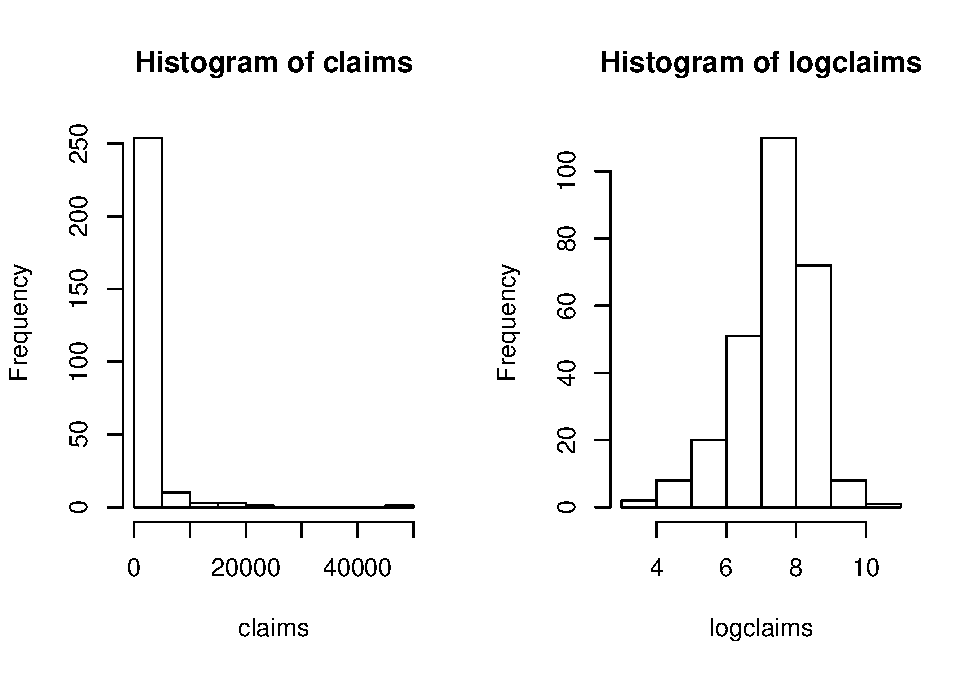
\includegraphics{RegressModelDataCamp_files/figure-latex/unnamed-chunk-18-1.pdf}

\subsection{Exercise. Visualizing bodily injury claims with density
plots}\label{exercise.-visualizing-bodily-injury-claims-with-density-plots}

\textbf{Assignment Text}

In the prior video, you learned about the Massachusetts bodily injury
dataset. This dataframe, \texttt{injury}, has been read in and the
global variable \texttt{claims} has been created. This assignment
reviews the
\href{https://www.rdocumentation.org/packages/graphics/versions/3.5.0/topics/hist/}{hist()}
function for visualizing distributions and allows you to explore density
plotting, a smoothed version of the histogram.

\textbf{Instructions}

\begin{itemize}
\tightlist
\item
  Use the function
  \href{https://www.rdocumentation.org/packages/base/versions/3.5.0/topics/log/}{log()}
  to create the logarithmic version of the claims variable
\item
  Calculate a histogram of logarithmic with 40 bins using an option in
  the
  \href{https://www.rdocumentation.org/packages/graphics/versions/3.5.0/topics/hist/}{hist()}
  function, \texttt{breaks\ =}.
\item
  Create a density plot of logarithmic claims using the functions
  \href{https://www.rdocumentation.org/packages/graphics/versions/3.5.0/topics/plot/}{plot()}
  and
  \href{https://www.rdocumentation.org/packages/stats/versions/3.5.0/topics/density/}{density()}.
\item
  Repeat the density plot, this time using a more refined bandwidth
  equal to 0.03. Use an option in the
  \href{https://www.rdocumentation.org/packages/stats/versions/3.5.0/topics/density/}{density()}
  function, \texttt{bw\ =}.
\end{itemize}

\textbf{Hint}

\textbf{Pre-exercise code}

\begin{Shaded}
\begin{Highlighting}[]
\CommentTok{# Pre-exercise code}
\NormalTok{injury <-}\StringTok{ }\KeywordTok{read.csv}\NormalTok{(}\StringTok{"CSVData}\CharTok{\textbackslash{}\textbackslash{}}\StringTok{MassBI.csv"}\NormalTok{,}\DataTypeTok{header =} \OtherTok{TRUE}\NormalTok{)}
\CommentTok{#injury <- read.csv("https://assets.datacamp.com/production/repositories/2610/datasets/8cca19d0503fcf6e9d30d9cb912de5ba95ecb9c1/MassBI.csv", header = TRUE)}
\NormalTok{claims <-}\StringTok{ }\NormalTok{injury}\OperatorTok{$}\NormalTok{claims}
\end{Highlighting}
\end{Shaded}

\textbf{SampleCode}

\begin{Shaded}
\begin{Highlighting}[]
\StringTok{`}\DataTypeTok{SampleCode}\StringTok{`}
\CommentTok{#Create the logarithmic claims variable}
\NormalTok{logclaims <-}\StringTok{ }\NormalTok{___}

\CommentTok{#Create a histogram usins 40 bins}
\KeywordTok{___}\NormalTok{(logclaims, }\DataTypeTok{breaks =} \DecValTok{40}\NormalTok{,}\DataTypeTok{freq =} \OtherTok{FALSE}\NormalTok{)}
\KeywordTok{box}\NormalTok{()}

\CommentTok{# Create a density plot of logarithmic claims}
\KeywordTok{plot}\NormalTok{(}\KeywordTok{___}\NormalTok{(logclaims))}

\CommentTok{# Create a density plot of logarithmic claims with a smaller bandwidth}
\NormalTok{___}
\end{Highlighting}
\end{Shaded}

\textbf{Solution}

\begin{Shaded}
\begin{Highlighting}[]
\CommentTok{# Solution}
\NormalTok{logclaims <-}\StringTok{ }\KeywordTok{log}\NormalTok{(claims)}
\KeywordTok{hist}\NormalTok{(logclaims , }\DataTypeTok{breaks =} \DecValTok{40}\NormalTok{,}\DataTypeTok{freq =} \OtherTok{FALSE}\NormalTok{)}
\KeywordTok{box}\NormalTok{()}
\end{Highlighting}
\end{Shaded}

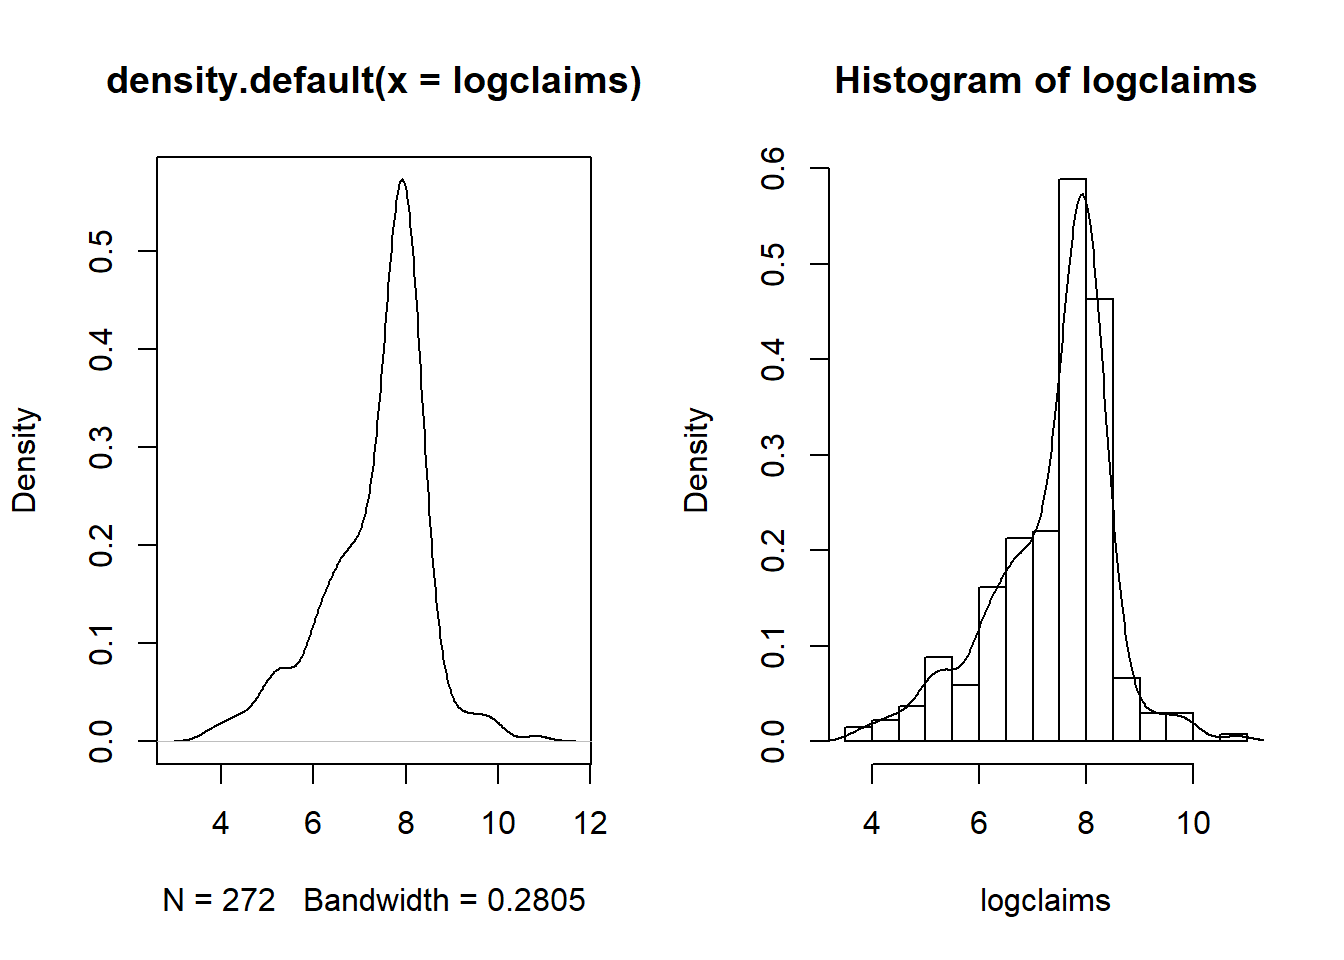
\includegraphics{RegressModelDataCamp_files/figure-latex/unnamed-chunk-21-1.pdf}

\begin{Shaded}
\begin{Highlighting}[]
\KeywordTok{plot}\NormalTok{(}\KeywordTok{density}\NormalTok{(logclaims))}
\end{Highlighting}
\end{Shaded}

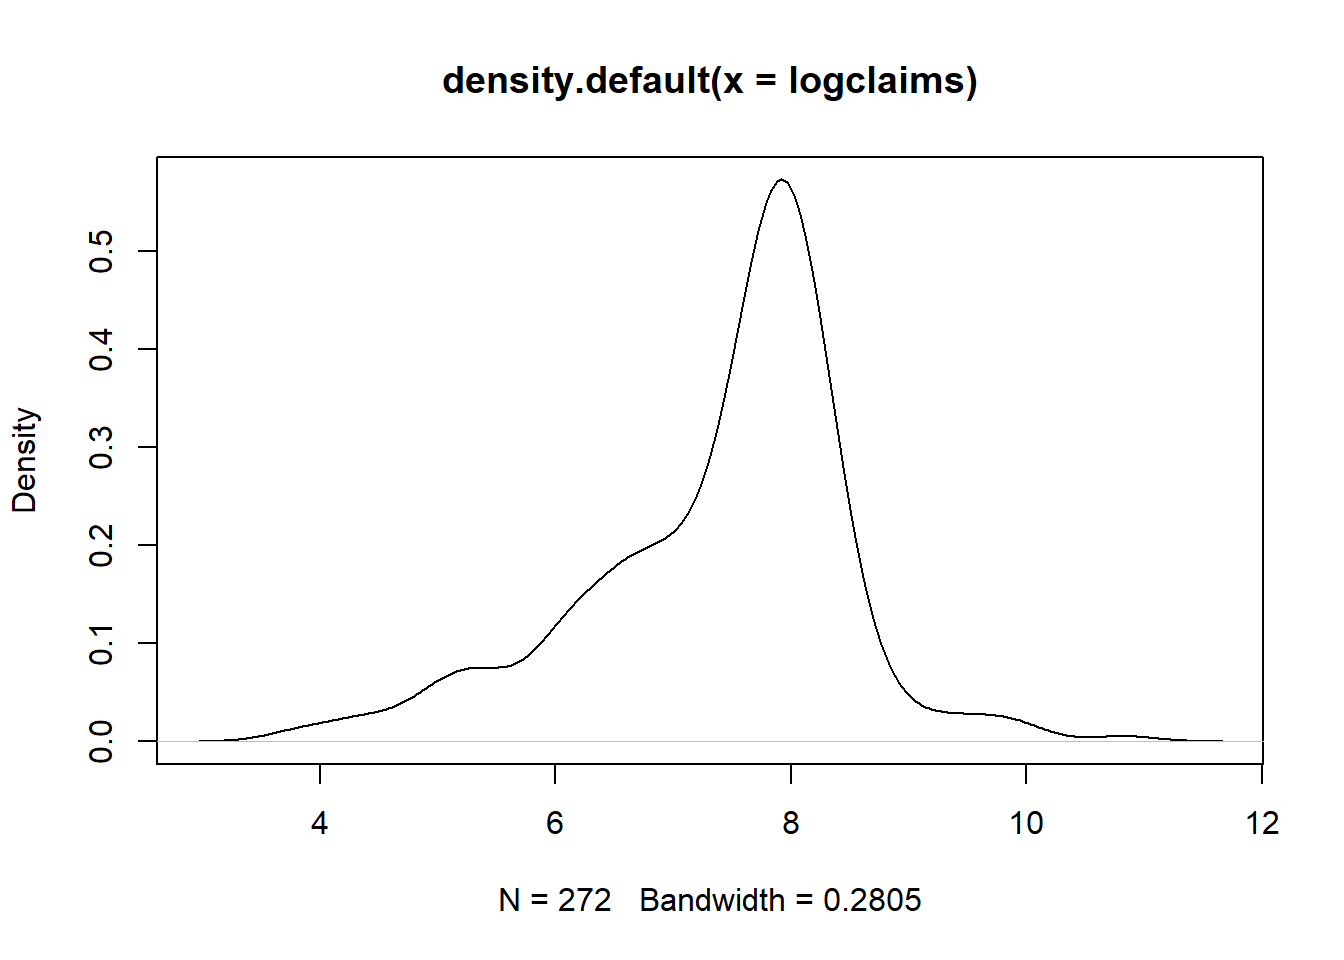
\includegraphics{RegressModelDataCamp_files/figure-latex/unnamed-chunk-21-2.pdf}

\begin{Shaded}
\begin{Highlighting}[]
\KeywordTok{plot}\NormalTok{(}\KeywordTok{density}\NormalTok{(logclaims, }\DataTypeTok{bw =} \FloatTok{0.03}\NormalTok{))}
\end{Highlighting}
\end{Shaded}

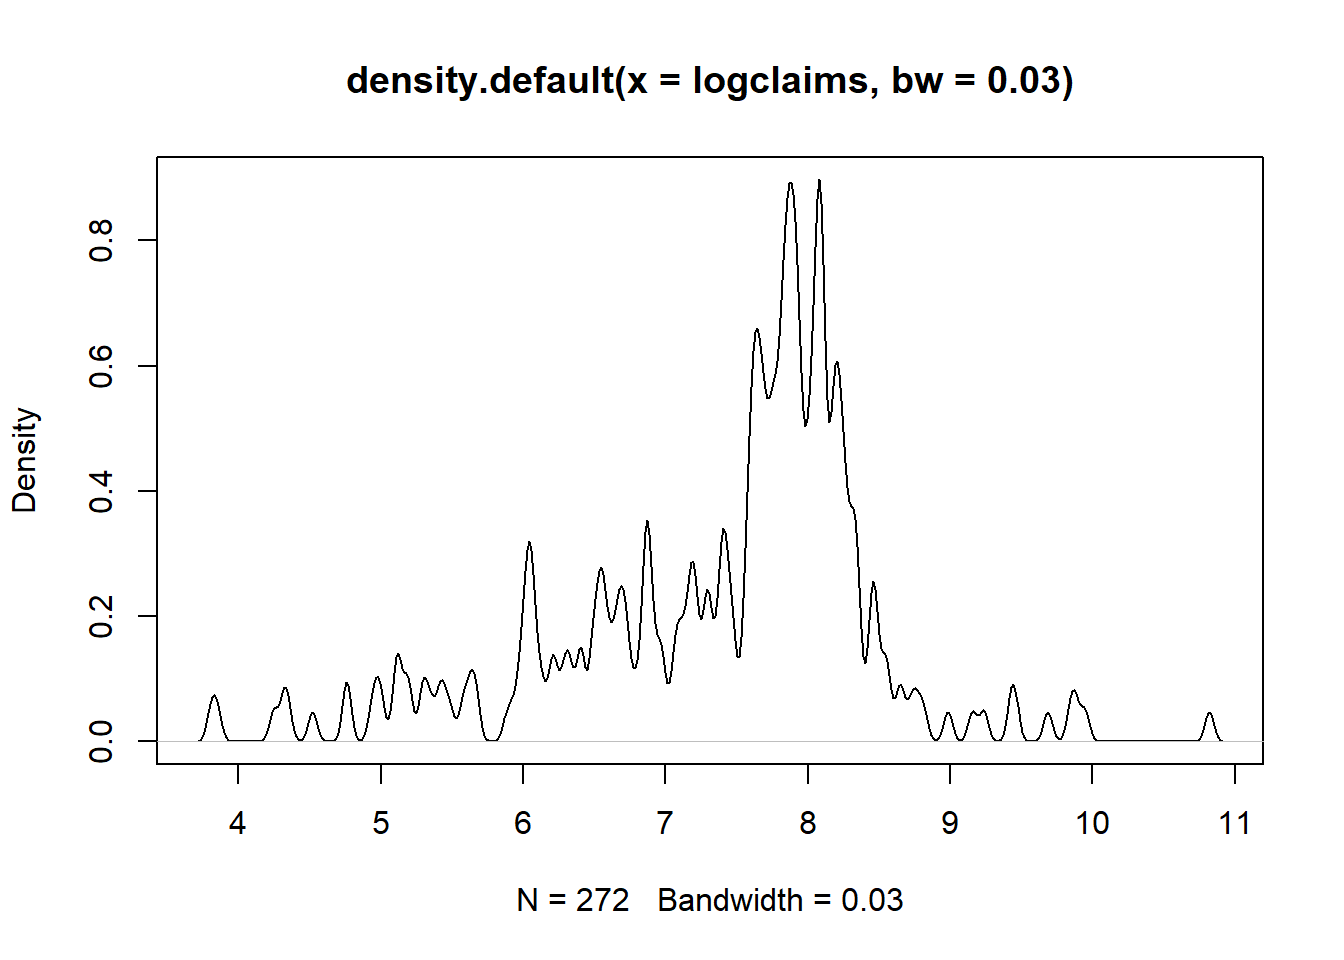
\includegraphics{RegressModelDataCamp_files/figure-latex/unnamed-chunk-21-3.pdf}

\textbf{Submission Correctness Tests (SCT)}

success\_msg(``Excellent! Visualizing the distribution is important and
smoothing techniques allow viewers to see important patterns without
being distracted by random fluctations.'')

\section{Summarizing distributions}\label{summarizing-distributions}

\subsection{Video (Exercise). Summarizing
distributions}\label{video-exercise.-summarizing-distributions}

\subsubsection{Learning Objectives}\label{learning-objectives-1}

In this section, you learn how to:

\begin{itemize}
\tightlist
\item
  Calculate and interpret basic summary statistics
\item
  Calculate and interpret distributions using boxplots
\item
  Calculate and interpret distributions using qq plots
\end{itemize}

\subsubsection{Video Overheads}\label{video-overheads}

\textbf{Overhead A. Summary Statistics}

\begin{Shaded}
\begin{Highlighting}[]
\NormalTok{injury <-}\StringTok{ }\KeywordTok{read.csv}\NormalTok{(}\StringTok{"CSVData}\CharTok{\textbackslash{}\textbackslash{}}\StringTok{MassBI.csv"}\NormalTok{,}\DataTypeTok{header =} \OtherTok{TRUE}\NormalTok{)}
\CommentTok{#injury <- read.csv("https://assets.datacamp.com/production/repositories/2610/datasets/8cca19d0503fcf6e9d30d9cb912de5ba95ecb9c1/MassBI.csv", header = TRUE)}
\KeywordTok{attach}\NormalTok{(injury)}

\CommentTok{# SUMMARY STATISTICS}
\KeywordTok{summary}\NormalTok{(injury)}
\KeywordTok{sd}\NormalTok{(claims);}\KeywordTok{sd}\NormalTok{(logclaims)}
\KeywordTok{length}\NormalTok{(claims)}
\end{Highlighting}
\end{Shaded}

\begin{verbatim}
     claims          logclaims     
 Min.   :   45.0   Min.   : 3.807  
 1st Qu.:  892.5   1st Qu.: 6.794  
 Median : 2210.0   Median : 7.701  
 Mean   : 2697.7   Mean   : 7.388  
 3rd Qu.: 3215.0   3rd Qu.: 8.076  
 Max.   :50000.0   Max.   :10.820  
[1] 3944.445
[1] 1.10093
[1] 272
\end{verbatim}

\textbf{Overhead B. Boxplot}

\begin{Shaded}
\begin{Highlighting}[]
\CommentTok{# BASIC BOXPLOT}
\KeywordTok{boxplot}\NormalTok{(logclaims)}
\end{Highlighting}
\end{Shaded}

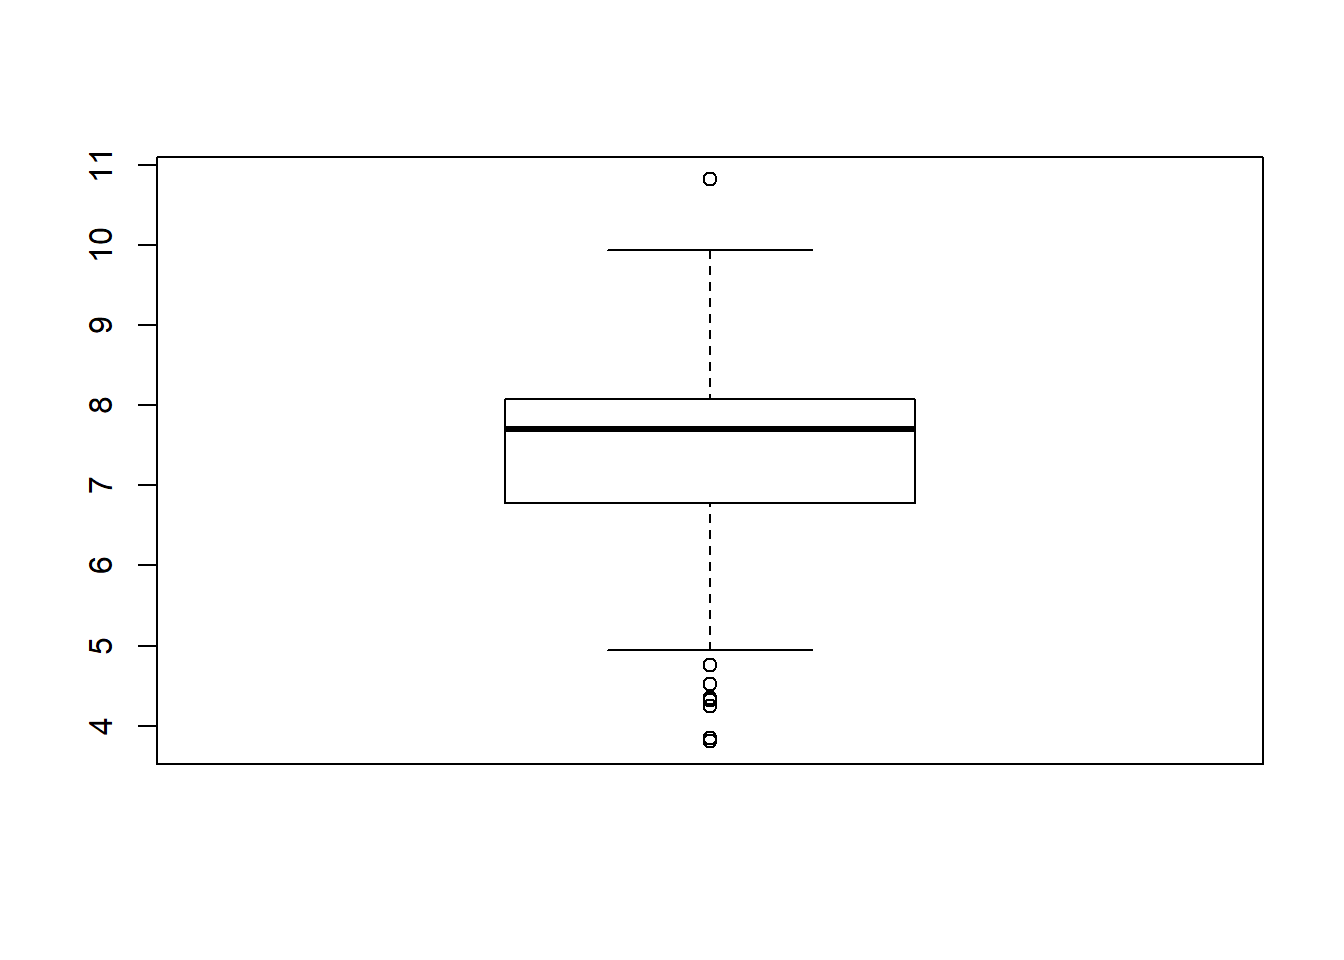
\includegraphics{RegressModelDataCamp_files/figure-latex/unnamed-chunk-23-1.pdf}

\begin{Shaded}
\begin{Highlighting}[]
\KeywordTok{quantile}\NormalTok{(logclaims, }\DataTypeTok{probs =} \FloatTok{0.75}\NormalTok{)}

\CommentTok{# BOXPLOT WITH ANNOTATION}
\KeywordTok{boxplot}\NormalTok{(logclaims, }\DataTypeTok{main =} \StringTok{"Boxplot of logclaims"}\NormalTok{)}
\KeywordTok{text}\NormalTok{(}\DecValTok{1}\NormalTok{,  }\FloatTok{7.6}\NormalTok{,  }\StringTok{"median"}\NormalTok{, }\DataTypeTok{cex =} \FloatTok{0.7}\NormalTok{)}
\KeywordTok{text}\NormalTok{(}\DecValTok{1}\NormalTok{,  }\FloatTok{6.55}\NormalTok{, }\StringTok{"25th percentile"}\NormalTok{, }\DataTypeTok{cex =} \FloatTok{0.7}\NormalTok{)}
\KeywordTok{text}\NormalTok{(}\DecValTok{1}\NormalTok{,  }\FloatTok{7.95}\NormalTok{, }\StringTok{"75th percentile"}\NormalTok{, }\DataTypeTok{cex =} \FloatTok{0.7}\NormalTok{)}
\KeywordTok{arrows}\NormalTok{(}\FloatTok{1.05}\NormalTok{, }\FloatTok{4.9}\NormalTok{, }\FloatTok{1.05}\NormalTok{, }\FloatTok{3.6}\NormalTok{, }\DataTypeTok{col =} \StringTok{"blue"}\NormalTok{, }\DataTypeTok{code =} \DecValTok{3}\NormalTok{, }\DataTypeTok{angle =} \DecValTok{20}\NormalTok{, }\DataTypeTok{length =} \FloatTok{0.1}\NormalTok{)}
\KeywordTok{text}\NormalTok{(}\FloatTok{1.1}\NormalTok{,  }\FloatTok{4.4}\NormalTok{, }\StringTok{"outliers"}\NormalTok{, }\DataTypeTok{cex =} \FloatTok{0.7}\NormalTok{)}
\KeywordTok{text}\NormalTok{(}\FloatTok{1.1}\NormalTok{, }\FloatTok{10.9}\NormalTok{, }\StringTok{"outlier"}\NormalTok{,  }\DataTypeTok{cex =} \FloatTok{0.7}\NormalTok{)}
\end{Highlighting}
\end{Shaded}

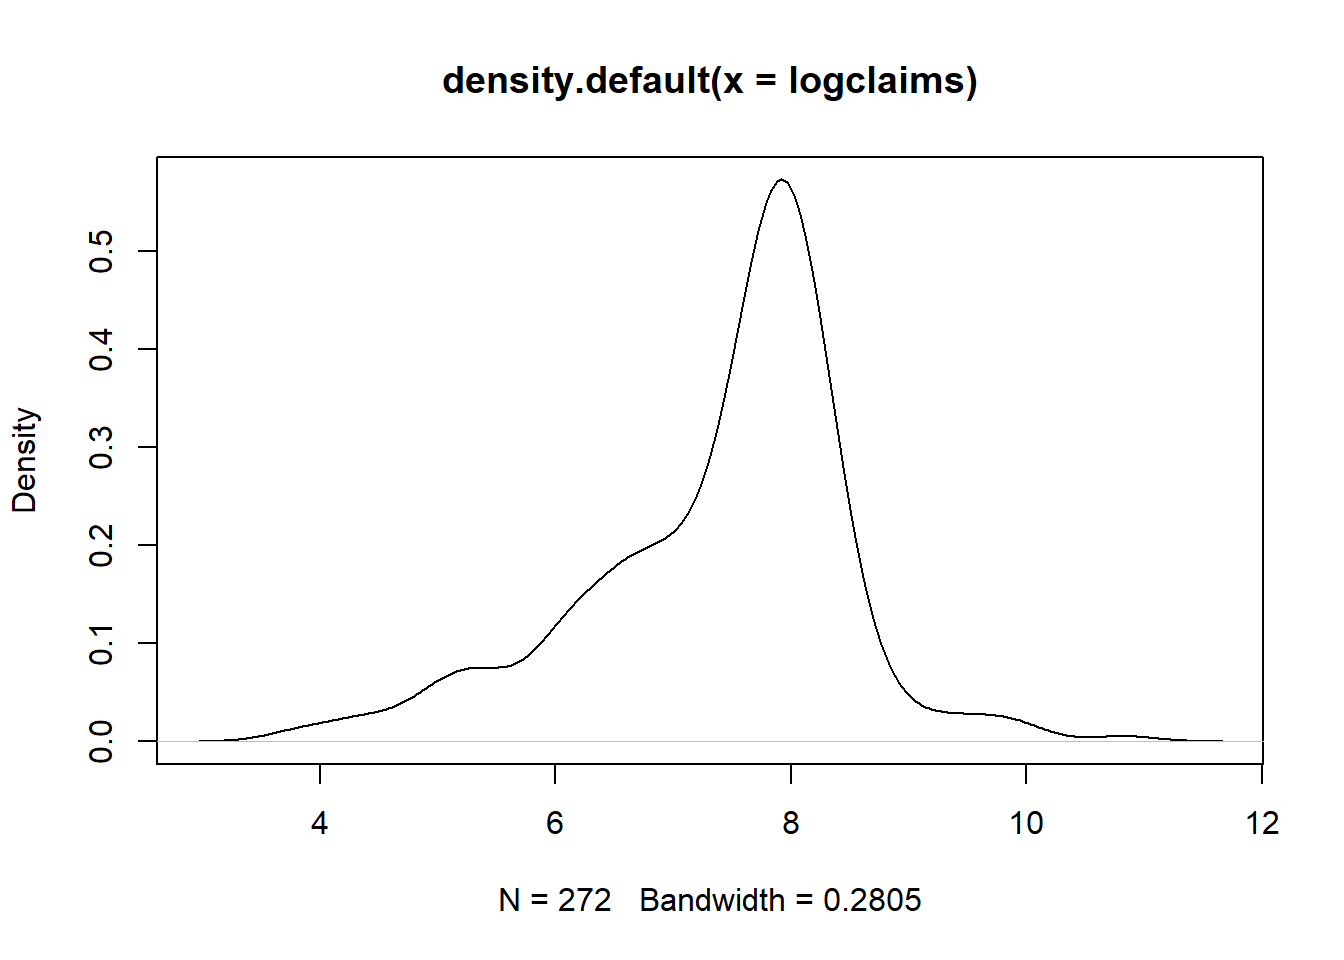
\includegraphics{RegressModelDataCamp_files/figure-latex/unnamed-chunk-23-2.pdf}

\begin{verbatim}
     75% 
8.075579 
\end{verbatim}

\textbf{Overhead C. QQ Plot}

\begin{Shaded}
\begin{Highlighting}[]
\KeywordTok{summary}\NormalTok{(injury)}
\KeywordTok{quantile}\NormalTok{(claims, }\DataTypeTok{probs =} \FloatTok{0.75}\NormalTok{)}
\KeywordTok{quantile}\NormalTok{(logclaims, }\DataTypeTok{probs =} \FloatTok{0.75}\NormalTok{)}
\KeywordTok{log}\NormalTok{(}\KeywordTok{quantile}\NormalTok{(claims, }\DataTypeTok{probs =} \FloatTok{0.75}\NormalTok{))}
\KeywordTok{qnorm}\NormalTok{(}\DataTypeTok{p =} \FloatTok{0.75}\NormalTok{, }\DataTypeTok{mean =} \KeywordTok{mean}\NormalTok{(logclaims), }\DataTypeTok{sd =} \KeywordTok{sd}\NormalTok{(logclaims))}
\NormalTok{(}\KeywordTok{qnorm}\NormalTok{(}\DataTypeTok{p =} \FloatTok{0.75}\NormalTok{, }\DataTypeTok{mean =} \KeywordTok{mean}\NormalTok{(logclaims), }\DataTypeTok{sd =} \KeywordTok{sd}\NormalTok{(logclaims)) }\OperatorTok{-}\KeywordTok{mean}\NormalTok{(logclaims)) }\OperatorTok{/}
\StringTok{       }\KeywordTok{sd}\NormalTok{(logclaims)}
\KeywordTok{qnorm}\NormalTok{(}\DataTypeTok{p =} \FloatTok{0.75}\NormalTok{, }\DataTypeTok{mean =} \DecValTok{0}\NormalTok{, }\DataTypeTok{sd =} \DecValTok{1}\NormalTok{)}

\CommentTok{#  QUANTILE - QUANTILE PLOT}
\KeywordTok{qqnorm}\NormalTok{(logclaims)}
\KeywordTok{qqline}\NormalTok{(logclaims)   }
\end{Highlighting}
\end{Shaded}

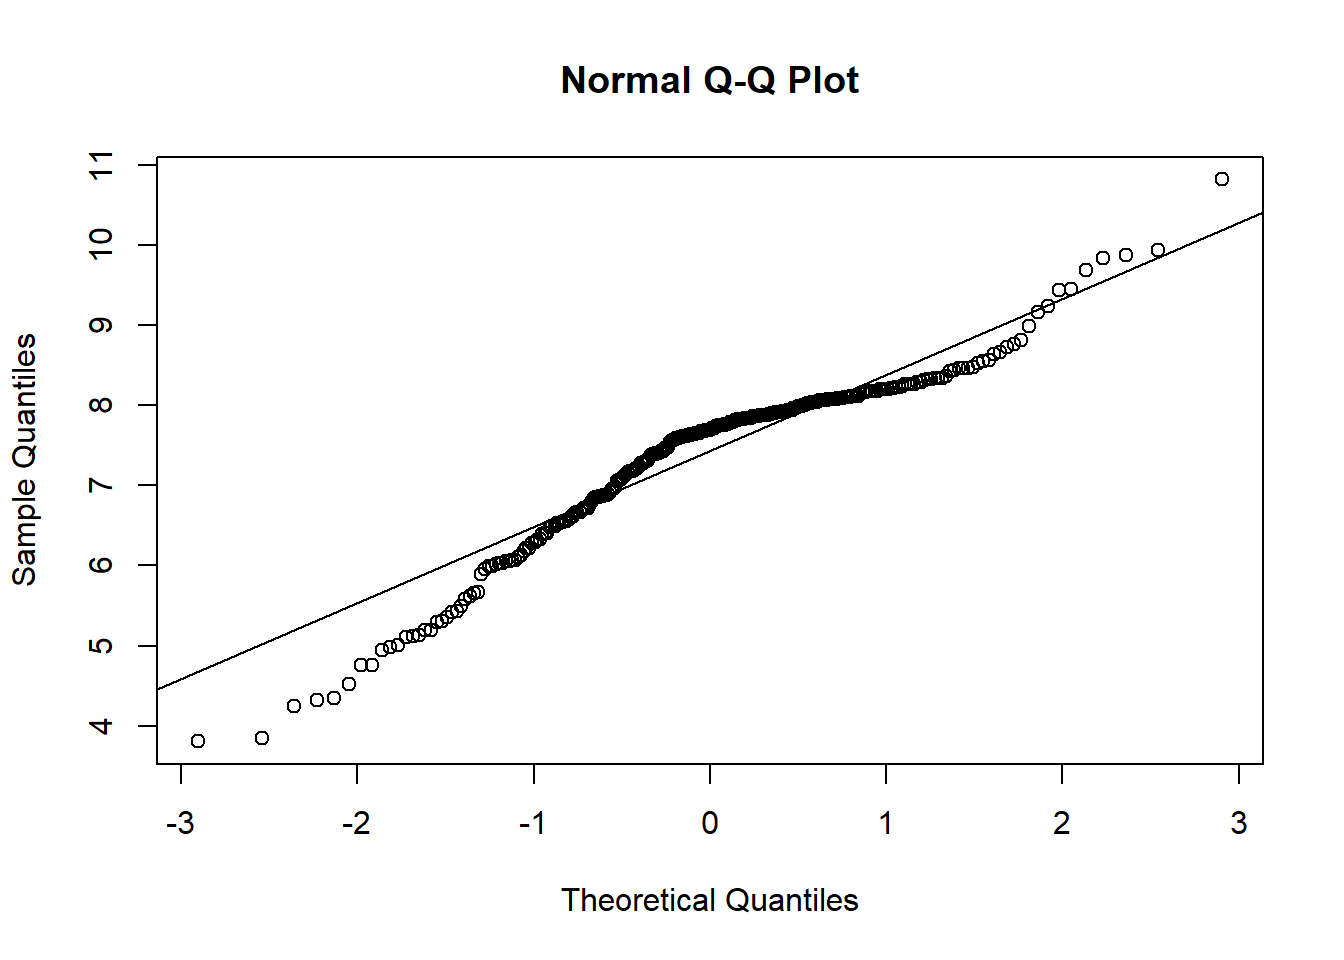
\includegraphics{RegressModelDataCamp_files/figure-latex/unnamed-chunk-24-1.pdf}

\begin{verbatim}
     claims          logclaims     
 Min.   :   45.0   Min.   : 3.807  
 1st Qu.:  892.5   1st Qu.: 6.794  
 Median : 2210.0   Median : 7.701  
 Mean   : 2697.7   Mean   : 7.388  
 3rd Qu.: 3215.0   3rd Qu.: 8.076  
 Max.   :50000.0   Max.   :10.820  
 75% 
3215 
     75% 
8.075579 
     75% 
8.075583 
[1] 8.131056
[1] 0.6744898
[1] 0.6744898
\end{verbatim}

\subsection{Exercise. Summarizing bodily injury claims with box and qq
plots}\label{exercise.-summarizing-bodily-injury-claims-with-box-and-qq-plots}

\textbf{Assignment Text}

The Massachusetts bodily injury data has already been read and used to
create the global variable \texttt{claims} representing bodily injury
claims. The previous video showed how to present the distribution of
logarithmic claims which appeared to be approximately normally
distributed. However, users are not really interested in log dollars but
want to know about a unit of measurement that is more intuitive, such as
dollars.

So this assignment is based on claims, not the logarithmic version. You
will use the functions
\href{https://www.rdocumentation.org/packages/graphics/versions/3.5.0/topics/boxplot/}{boxplot()}
and
\href{https://www.rdocumentation.org/packages/stats/versions/3.5.0/topics/qqnorm/}{qqnorm()}
to visualize the distribution through boxplots and quantile-quantile, or
qq-, plots. But, because we are working with such a skewed distribution,
do not be surprised that it is difficult to interpret these results
readily.

\textbf{Instructions}

\begin{itemize}
\tightlist
\item
  Produce a box plot for claims
\item
  Determine the 25th empirical percentile for claims using the
  \href{https://www.rdocumentation.org/packages/stats/versions/3.5.0/topics/quantile/}{quantile()}
  function.
\item
  Determine the 25th percentile for claims based on a normal
  distribution using the
  \href{https://www.rdocumentation.org/packages/stats/versions/3.5.0/topics/Normal/}{qnorm()}
  function.
\item
  Produce a normal qq plot for claims using the function
  \href{https://www.rdocumentation.org/packages/stats/versions/3.5.0/topics/qqnorm/}{qqnorm()}.
  The
  \href{https://www.rdocumentation.org/packages/stats/versions/3.5.0/topics/qqnorm/}{qqline()}
  function is handy for producing a reference line.
\end{itemize}

\textbf{Hint}

Note that
\href{https://www.rdocumentation.org/packages/stats/versions/3.5.0/topics/Normal/}{qnorm()}
(one \texttt{q}) is for a normal quantile and
\href{https://www.rdocumentation.org/packages/stats/versions/3.5.0/topics/qqnorm/}{qqnorm()}.
(two \texttt{q}'s!) is for the normal qq plot

\textbf{Pre-exercise code}

\begin{Shaded}
\begin{Highlighting}[]
\CommentTok{# Pre-exercise code}
\NormalTok{injury <-}\StringTok{ }\KeywordTok{read.csv}\NormalTok{(}\StringTok{"CSVData}\CharTok{\textbackslash{}\textbackslash{}}\StringTok{MassBI.csv"}\NormalTok{, }\DataTypeTok{header =} \OtherTok{TRUE}\NormalTok{)}
\CommentTok{#injury <- read.csv("https://assets.datacamp.com/production/repositories/2610/datasets/8cca19d0503fcf6e9d30d9cb912de5ba95ecb9c1/MassBI.csv", header = TRUE)}
\NormalTok{claims <-}\StringTok{ }\NormalTok{injury}\OperatorTok{$}\NormalTok{claims}
\end{Highlighting}
\end{Shaded}

\textbf{SampleCode}

\begin{Shaded}
\begin{Highlighting}[]
\StringTok{`}\DataTypeTok{SampleCode}\StringTok{`}
\CommentTok{#Produce a box plot for claims}
\KeywordTok{___}\NormalTok{(claims)}

\CommentTok{#Determine the 25th empirical percentile for claims}
\NormalTok{q25 <-}\StringTok{ }\KeywordTok{___}\NormalTok{(claims, }\DataTypeTok{probs =}\NormalTok{ ___)}
\NormalTok{q25}

\CommentTok{#Determine the 25th percentile for claims based on a normal distribution}
\NormalTok{qn25 <-}\StringTok{ }\KeywordTok{___}\NormalTok{(}\DataTypeTok{p =}\NormalTok{ ___, }\DataTypeTok{mean =} \KeywordTok{mean}\NormalTok{(claims), }\DataTypeTok{sd =} \KeywordTok{sd}\NormalTok{(claims))}
\NormalTok{qn25}

\CommentTok{#Produce a normal qq plot for claims}
\KeywordTok{___}\NormalTok{(claims)}
\KeywordTok{___}\NormalTok{(claims)}
\end{Highlighting}
\end{Shaded}

\textbf{Solution}

\begin{Shaded}
\begin{Highlighting}[]
\CommentTok{# Solution}
\KeywordTok{boxplot}\NormalTok{(claims)}
\end{Highlighting}
\end{Shaded}

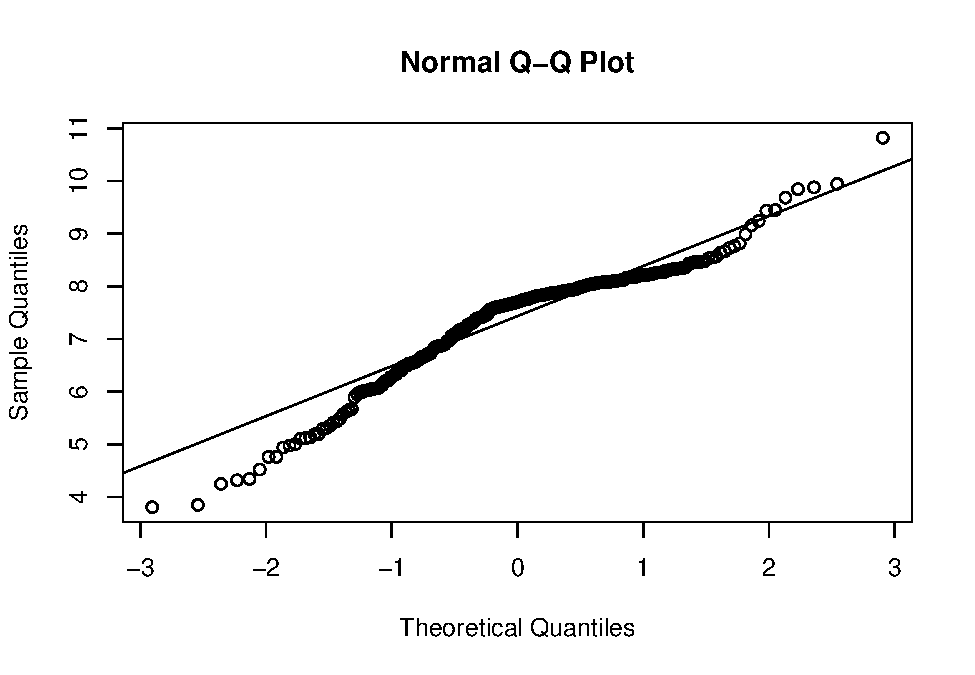
\includegraphics{RegressModelDataCamp_files/figure-latex/unnamed-chunk-27-1.pdf}

\begin{Shaded}
\begin{Highlighting}[]
\NormalTok{q25 <-}\StringTok{ }\KeywordTok{quantile}\NormalTok{(claims, }\DataTypeTok{probs =} \FloatTok{0.25}\NormalTok{)}
\NormalTok{q25}
\NormalTok{qn25 <-}\StringTok{ }\KeywordTok{qnorm}\NormalTok{(}\DataTypeTok{p =} \FloatTok{0.25}\NormalTok{, }\DataTypeTok{mean =} \KeywordTok{mean}\NormalTok{(claims), }\DataTypeTok{sd =} \KeywordTok{sd}\NormalTok{(claims))}
\NormalTok{qn25}
\KeywordTok{qqnorm}\NormalTok{(claims)}
\KeywordTok{qqline}\NormalTok{(claims)   }
\end{Highlighting}
\end{Shaded}

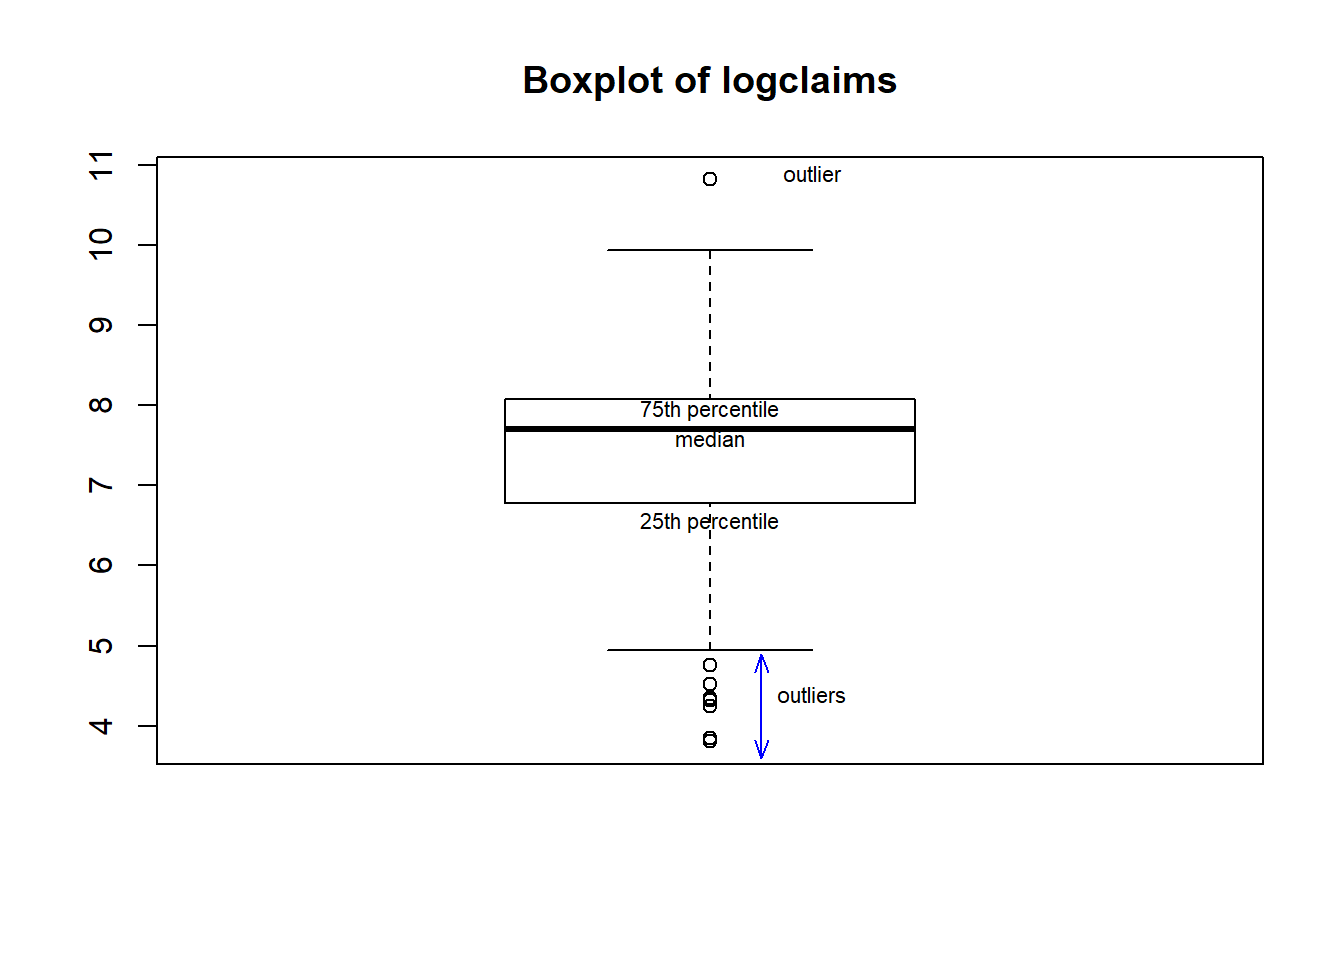
\includegraphics{RegressModelDataCamp_files/figure-latex/unnamed-chunk-27-2.pdf}

\begin{verbatim}
  25% 
892.5 
[1] 37.22942
\end{verbatim}

\textbf{Submission Correctness Tests (SCT)}

test\_error() test\_object(``q25'', incorrect\_msg = ``You calculated
the 25th quantile incorrectly. Check out the quantile() function.'')
test\_object(``qn25'', incorrect\_msg = ``You calculated the 25th
quantile incorrectly. Check out the qnorm() function.'')
success\_msg(``Congratulations on learning about box and qq plots.
Although you are unlikely to show these plots to consumers of your
analysis, you will find them useful tools for exploring multivariate
aspects of data.'')

\subsection{Exercise. Effects on distributions of removing the largest
claim}\label{exercise.-effects-on-distributions-of-removing-the-largest-claim}

\textbf{Assignment Text}

The Massachusetts bodily injury dataframe \texttt{injury} has been read
in; our focus is on the \texttt{claims} variable in that dataset.

In the previous exercise, we learned that the Massachusetts bodily
injury \texttt{claims} distribution was not even close to approximately
normal (as evidenced by the box and qq- plots). Non-normality may be
induced by skewness (that we will handle via transformations in the next
section). But, seeming non-normality can also be induced by one or two
very large observations (called an \emph{outlier} later in the course).
So, this exercise examines the effects on the distribution of removing
the largest claims.

\textbf{Instructions}

\begin{itemize}
\tightlist
\item
  Use the function
  \href{https://www.rdocumentation.org/packages/utils/versions/3.5.0/topics/head}{tail()}
  to examine the \texttt{injury} dataset and identify the largest claim
\item
  Use the function
  \href{https://www.rdocumentation.org/packages/base/versions/3.5.0/topics/subset}{subset()}
  to create a subset omitting the largest claim
\item
  Compare the summary statistics of the omitted claim distribution to
  the full distribution
\item
  Compare the two distributions visually via histograms plotted next to
  another. \texttt{par(mfrow\ =\ c(1,\ 2))} is used to organize the
  plots you create. Do not alter this code.
\end{itemize}

\textbf{Hint}

For this data set, the {[}subset(){]} argument
\texttt{claims\ \textless{}\ 25000} will keep all but the largest claim

\textbf{Pre-exercise code}

\begin{Shaded}
\begin{Highlighting}[]
\CommentTok{# Pre-exercise code}
\NormalTok{injury <-}\StringTok{ }\KeywordTok{read.csv}\NormalTok{(}\StringTok{"CSVData}\CharTok{\textbackslash{}\textbackslash{}}\StringTok{MassBI.csv"}\NormalTok{, }\DataTypeTok{header =} \OtherTok{TRUE}\NormalTok{)}
\CommentTok{#injury <- read.csv("https://assets.datacamp.com/production/repositories/2610/datasets/8cca19d0503fcf6e9d30d9cb912de5ba95ecb9c1/MassBI.csv", header = TRUE)}
\NormalTok{claims <-}\StringTok{ }\NormalTok{injury}\OperatorTok{$}\NormalTok{claims}
\end{Highlighting}
\end{Shaded}

\textbf{SampleCode}

\begin{Shaded}
\begin{Highlighting}[]
\StringTok{`}\DataTypeTok{SampleCode}\StringTok{`}
\CommentTok{# Examine the tail of the `injury` dataset}
\KeywordTok{tail}\NormalTok{(___)}

\CommentTok{# Create a subset omitting the largest claim}
\NormalTok{injury2 <-}\StringTok{ }\KeywordTok{subset}\NormalTok{(injury, ___)}

\CommentTok{# Compare the summary statistics of the omitted claim distribution to the full distribution}
\KeywordTok{summary}\NormalTok{(___)}
\KeywordTok{summary}\NormalTok{(injury2)}

\CommentTok{# Compare the two distributions visually via histograms plotted next to another}
\KeywordTok{par}\NormalTok{(}\DataTypeTok{mfrow =} \KeywordTok{c}\NormalTok{(}\DecValTok{1}\NormalTok{, }\DecValTok{2}\NormalTok{))}
\KeywordTok{hist}\NormalTok{(___, }\DataTypeTok{freq =} \OtherTok{FALSE}\NormalTok{,  }\DataTypeTok{main =} \StringTok{"Full Data"}\NormalTok{)}
\KeywordTok{hist}\NormalTok{(___, }\DataTypeTok{freq =} \OtherTok{FALSE}\NormalTok{,  }\DataTypeTok{main =} \StringTok{"Largest Claim Omitted"}\NormalTok{)}
\end{Highlighting}
\end{Shaded}

\textbf{Solution}

\begin{Shaded}
\begin{Highlighting}[]
\CommentTok{# Solution}
\KeywordTok{tail}\NormalTok{(injury)}
\NormalTok{injury2 <-}\StringTok{ }\KeywordTok{subset}\NormalTok{(injury, claims }\OperatorTok{<}\StringTok{ }\DecValTok{25000}\NormalTok{ )}
\KeywordTok{summary}\NormalTok{(injury)}
\KeywordTok{summary}\NormalTok{(injury2)}

\KeywordTok{par}\NormalTok{(}\DataTypeTok{mfrow =} \KeywordTok{c}\NormalTok{(}\DecValTok{1}\NormalTok{, }\DecValTok{2}\NormalTok{))}
\KeywordTok{hist}\NormalTok{(claims, }\DataTypeTok{freq =} \OtherTok{FALSE}\NormalTok{,  }\DataTypeTok{main =} \StringTok{"Full Data"}\NormalTok{)}
\KeywordTok{hist}\NormalTok{(injury2}\OperatorTok{$}\NormalTok{claims, }\DataTypeTok{freq =} \OtherTok{FALSE}\NormalTok{,  }\DataTypeTok{main =} \StringTok{"Largest Claim Omitted"}\NormalTok{)}
\end{Highlighting}
\end{Shaded}

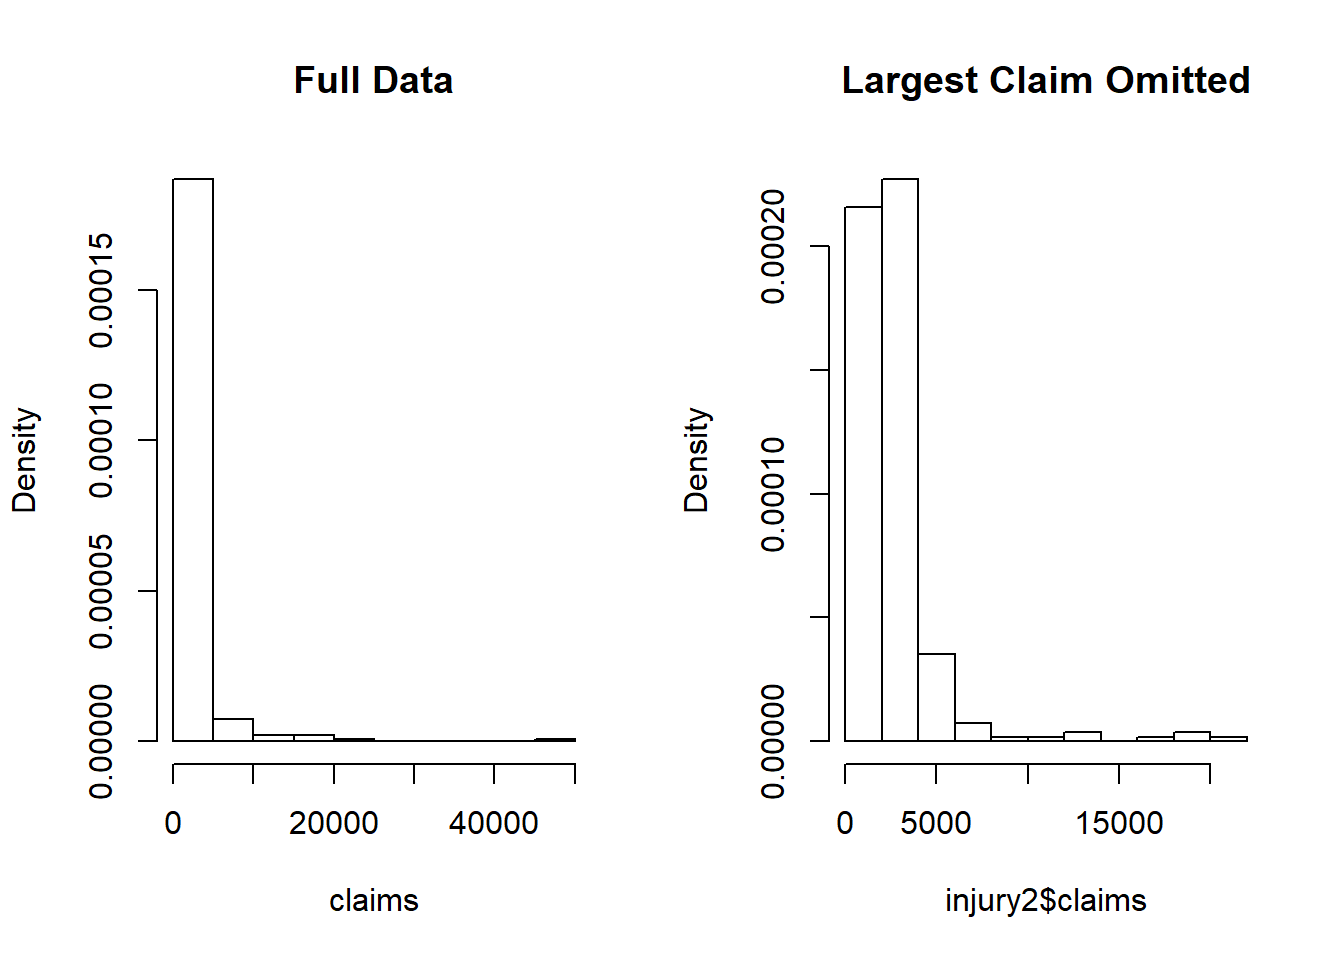
\includegraphics{RegressModelDataCamp_files/figure-latex/unnamed-chunk-30-1.pdf}

\begin{verbatim}
    claims logclaims
267  12688  9.448412
268  16043  9.683028
269  18847  9.844109
270  19500  9.878170
271  20827  9.944006
272  50000 10.819778
     claims          logclaims     
 Min.   :   45.0   Min.   : 3.807  
 1st Qu.:  892.5   1st Qu.: 6.794  
 Median : 2210.0   Median : 7.701  
 Mean   : 2697.7   Mean   : 7.388  
 3rd Qu.: 3215.0   3rd Qu.: 8.076  
 Max.   :50000.0   Max.   :10.820  
     claims        logclaims    
 Min.   :   45   Min.   :3.807  
 1st Qu.:  885   1st Qu.:6.785  
 Median : 2196   Median :7.694  
 Mean   : 2523   Mean   :7.376  
 3rd Qu.: 3205   3rd Qu.:8.072  
 Max.   :20827   Max.   :9.944  
\end{verbatim}

\textbf{Submission Correctness Tests (SCT)}

test\_error() test\_object(``injury2'', incorrect\_msg = ``You defined
the \texttt{injury} dataframe incorrectly. Check out the subset function
(and maybe look over the hint).'') success\_msg(``Congratulations! The
goal of predictive modeling is to discover patterns in the data.
However, sometimes seeming `patterns' are the result of one or two
unusual observations. Unusual observations may be due to incorrect data
gathering procedures or just due to wild fluctuations in a process of
interest but are common in predictive modeling.'')

\section{Transformations}\label{transformations}

\subsection{Video (Exercise).
Transformations}\label{video-exercise.-transformations}

\subsubsection{Learning Objectives}\label{learning-objectives-2}

In this exercise, you learn how to:

\begin{itemize}
\tightlist
\item
  Symmetrize a skewed distribution using a logarithmic transformation
\end{itemize}

\subsubsection{Video Overheads}\label{video-overheads-1}

\textbf{Overhead A. Simulate a moderately skewed distribution, with
transforms}

\begin{Shaded}
\begin{Highlighting}[]
\CommentTok{#  FIGURE 1.7 - SIMULATE CHI-SQUARE, CREATE 3 TRANSFORMATIONS}
\KeywordTok{set.seed}\NormalTok{(}\DecValTok{1237}\NormalTok{)                  }\CommentTok{# set the seed of the random number generator}
                                \CommentTok{# allows us to replicate results}
\NormalTok{X1 <-}\StringTok{ }\DecValTok{10000}\OperatorTok{*}\KeywordTok{rchisq}\NormalTok{(}\DecValTok{500}\NormalTok{, }\DataTypeTok{df =} \DecValTok{2}\NormalTok{) }\CommentTok{# generate variables randomly from a skewed distribution}
\NormalTok{X2 <-}\StringTok{ }\NormalTok{X1}\OperatorTok{^}\NormalTok{(}\FloatTok{0.5}\NormalTok{)                  }\CommentTok{# square root transform, could also use sqrt(X1)}
\NormalTok{X3 <-}\StringTok{ }\KeywordTok{log}\NormalTok{(X1)                   }\CommentTok{# logarithmic transform}
\NormalTok{X4 <-}\StringTok{ }\OperatorTok{-}\DecValTok{1}\OperatorTok{/}\NormalTok{X1                     }\CommentTok{# negative reciprocal transform}
\end{Highlighting}
\end{Shaded}

\textbf{Overhead B. Visualize the distributions}

\begin{Shaded}
\begin{Highlighting}[]
\KeywordTok{par}\NormalTok{(}\DataTypeTok{mfrow =} \KeywordTok{c}\NormalTok{(}\DecValTok{2}\NormalTok{, }\DecValTok{2}\NormalTok{), }\DataTypeTok{cex =}\NormalTok{ .}\DecValTok{75}\NormalTok{, }\DataTypeTok{mar =} \KeywordTok{c}\NormalTok{(}\DecValTok{3}\NormalTok{,}\DecValTok{5}\NormalTok{,}\FloatTok{1.5}\NormalTok{,}\DecValTok{0}\NormalTok{))}
\KeywordTok{hist}\NormalTok{(X1, }\DataTypeTok{freq =} \OtherTok{FALSE}\NormalTok{,  }\DataTypeTok{nclass =} \DecValTok{16}\NormalTok{, }\DataTypeTok{main =} \StringTok{""}\NormalTok{, }\DataTypeTok{xlab =} \StringTok{""}\NormalTok{, }\DataTypeTok{ylab =} \StringTok{""}\NormalTok{, }
      \DataTypeTok{las =} \DecValTok{1}\NormalTok{, }\DataTypeTok{yaxt =} \StringTok{"n"}\NormalTok{,}\DataTypeTok{xlim =} \KeywordTok{c}\NormalTok{(}\DecValTok{0}\NormalTok{,}\DecValTok{200000}\NormalTok{),}\DataTypeTok{ylim =} \KeywordTok{c}\NormalTok{(}\DecValTok{0}\NormalTok{,.}\DecValTok{00005}\NormalTok{))}
\KeywordTok{axis}\NormalTok{(}\DecValTok{2}\NormalTok{, }\DataTypeTok{at =} \KeywordTok{seq}\NormalTok{(}\DecValTok{0}\NormalTok{,.}\DecValTok{00005}\NormalTok{,.}\DecValTok{00001}\NormalTok{),}\DataTypeTok{las =} \DecValTok{1}\NormalTok{, }\DataTypeTok{cex =}\NormalTok{ .}\DecValTok{3}\NormalTok{, }
  \DataTypeTok{labels =} \KeywordTok{c}\NormalTok{(}\StringTok{"0"}\NormalTok{, }\StringTok{"0.00001"}\NormalTok{, }\StringTok{"0.00002"}\NormalTok{,}\StringTok{"0.00003"}\NormalTok{, }\StringTok{"0.00004"}\NormalTok{, }\StringTok{"0.00005"}\NormalTok{))}
\KeywordTok{mtext}\NormalTok{(}\StringTok{"Density"}\NormalTok{, }\DataTypeTok{side =} \DecValTok{2}\NormalTok{, }\DataTypeTok{at =}\NormalTok{ .}\DecValTok{000055}\NormalTok{, }\DataTypeTok{las =} \DecValTok{1}\NormalTok{, }\DataTypeTok{cex =}\NormalTok{ .}\DecValTok{75}\NormalTok{)}
\KeywordTok{mtext}\NormalTok{(}\StringTok{"y"}\NormalTok{, }\DataTypeTok{side =} \DecValTok{1}\NormalTok{, }\DataTypeTok{cex =}\NormalTok{ .}\DecValTok{75}\NormalTok{, }\DataTypeTok{line =} \DecValTok{2}\NormalTok{)}

\KeywordTok{par}\NormalTok{(}\DataTypeTok{mar =} \KeywordTok{c}\NormalTok{(}\DecValTok{3}\NormalTok{,}\DecValTok{4}\NormalTok{,}\FloatTok{1.5}\NormalTok{,}\FloatTok{0.2}\NormalTok{))}
\KeywordTok{hist}\NormalTok{(X2, }\DataTypeTok{freq =} \OtherTok{FALSE}\NormalTok{,  }\DataTypeTok{nclass =} \DecValTok{16}\NormalTok{, }\DataTypeTok{main =} \StringTok{""}\NormalTok{, }\DataTypeTok{xlab =} \StringTok{""}\NormalTok{, }\DataTypeTok{ylab =} \StringTok{""}\NormalTok{, }
      \DataTypeTok{las =} \DecValTok{1}\NormalTok{,}\DataTypeTok{xlim =} \KeywordTok{c}\NormalTok{(}\DecValTok{0}\NormalTok{,}\DecValTok{400}\NormalTok{), }\DataTypeTok{ylim =} \KeywordTok{c}\NormalTok{(}\DecValTok{0}\NormalTok{,.}\DecValTok{008}\NormalTok{))}
\KeywordTok{mtext}\NormalTok{(}\StringTok{"Density"}\NormalTok{, }\DataTypeTok{side =} \DecValTok{2}\NormalTok{, }\DataTypeTok{at =}\NormalTok{ .}\DecValTok{0088}\NormalTok{, }\DataTypeTok{las =} \DecValTok{1}\NormalTok{, }\DataTypeTok{cex =}\NormalTok{ .}\DecValTok{75}\NormalTok{)}
\KeywordTok{mtext}\NormalTok{(}\StringTok{"Square root of y"}\NormalTok{, }\DataTypeTok{side =} \DecValTok{1}\NormalTok{, }\DataTypeTok{cex =}\NormalTok{ .}\DecValTok{75}\NormalTok{, }\DataTypeTok{line =} \DecValTok{2}\NormalTok{)}

\KeywordTok{par}\NormalTok{(}\DataTypeTok{mar =} \KeywordTok{c}\NormalTok{(}\FloatTok{3.2}\NormalTok{,}\DecValTok{5}\NormalTok{,}\DecValTok{1}\NormalTok{,}\DecValTok{0}\NormalTok{))}
\KeywordTok{hist}\NormalTok{(X3,  }\DataTypeTok{freq =} \OtherTok{FALSE}\NormalTok{,  }\DataTypeTok{nclass =} \DecValTok{16}\NormalTok{, }\DataTypeTok{main =} \StringTok{""}\NormalTok{, }\DataTypeTok{xlab =} \StringTok{""}\NormalTok{, }\DataTypeTok{ylab =} \StringTok{""}\NormalTok{, }\DataTypeTok{las =} \DecValTok{1}\NormalTok{, }\DataTypeTok{ylim =} \KeywordTok{c}\NormalTok{(}\DecValTok{0}\NormalTok{,.}\DecValTok{4}\NormalTok{))}
\KeywordTok{mtext}\NormalTok{(}\StringTok{"Density"}\NormalTok{, }\DataTypeTok{side =} \DecValTok{2}\NormalTok{, }\DataTypeTok{at =}\NormalTok{ .}\DecValTok{44}\NormalTok{, }\DataTypeTok{las =} \DecValTok{1}\NormalTok{, }\DataTypeTok{cex =}\NormalTok{ .}\DecValTok{75}\NormalTok{)}
\KeywordTok{mtext}\NormalTok{(}\StringTok{"Logarithmic y"}\NormalTok{, }\DataTypeTok{side =} \DecValTok{1}\NormalTok{, }\DataTypeTok{cex =}\NormalTok{ .}\DecValTok{75}\NormalTok{, }\DataTypeTok{line =} \DecValTok{2}\NormalTok{)}

\KeywordTok{par}\NormalTok{(}\DataTypeTok{mar =} \KeywordTok{c}\NormalTok{(}\FloatTok{3.2}\NormalTok{,}\DecValTok{4}\NormalTok{,}\DecValTok{1}\NormalTok{,}\FloatTok{0.2}\NormalTok{))}
\KeywordTok{hist}\NormalTok{(X4, }\DataTypeTok{freq =} \OtherTok{FALSE}\NormalTok{,  }\DataTypeTok{nclass =} \DecValTok{16}\NormalTok{, }\DataTypeTok{main =} \StringTok{""}\NormalTok{,}\DataTypeTok{xlab =} \StringTok{""}\NormalTok{, }\DataTypeTok{ylab =} \StringTok{""}\NormalTok{, }\DataTypeTok{las =} \DecValTok{1}\NormalTok{, }\DataTypeTok{ylim =} \KeywordTok{c}\NormalTok{(}\DecValTok{0}\NormalTok{,}\DecValTok{100}\NormalTok{))}
\KeywordTok{mtext}\NormalTok{(}\StringTok{"Density"}\NormalTok{, }\DataTypeTok{side =} \DecValTok{2}\NormalTok{, }\DataTypeTok{at =} \DecValTok{110}\NormalTok{, }\DataTypeTok{las =} \DecValTok{1}\NormalTok{, }\DataTypeTok{cex =}\NormalTok{ .}\DecValTok{75}\NormalTok{)}
\KeywordTok{mtext}\NormalTok{(}\StringTok{"Negative reciprocal of y"}\NormalTok{, }\DataTypeTok{side =} \DecValTok{1}\NormalTok{, }\DataTypeTok{cex =}\NormalTok{ .}\DecValTok{75}\NormalTok{, }\DataTypeTok{line =} \DecValTok{2}\NormalTok{)}
\end{Highlighting}
\end{Shaded}

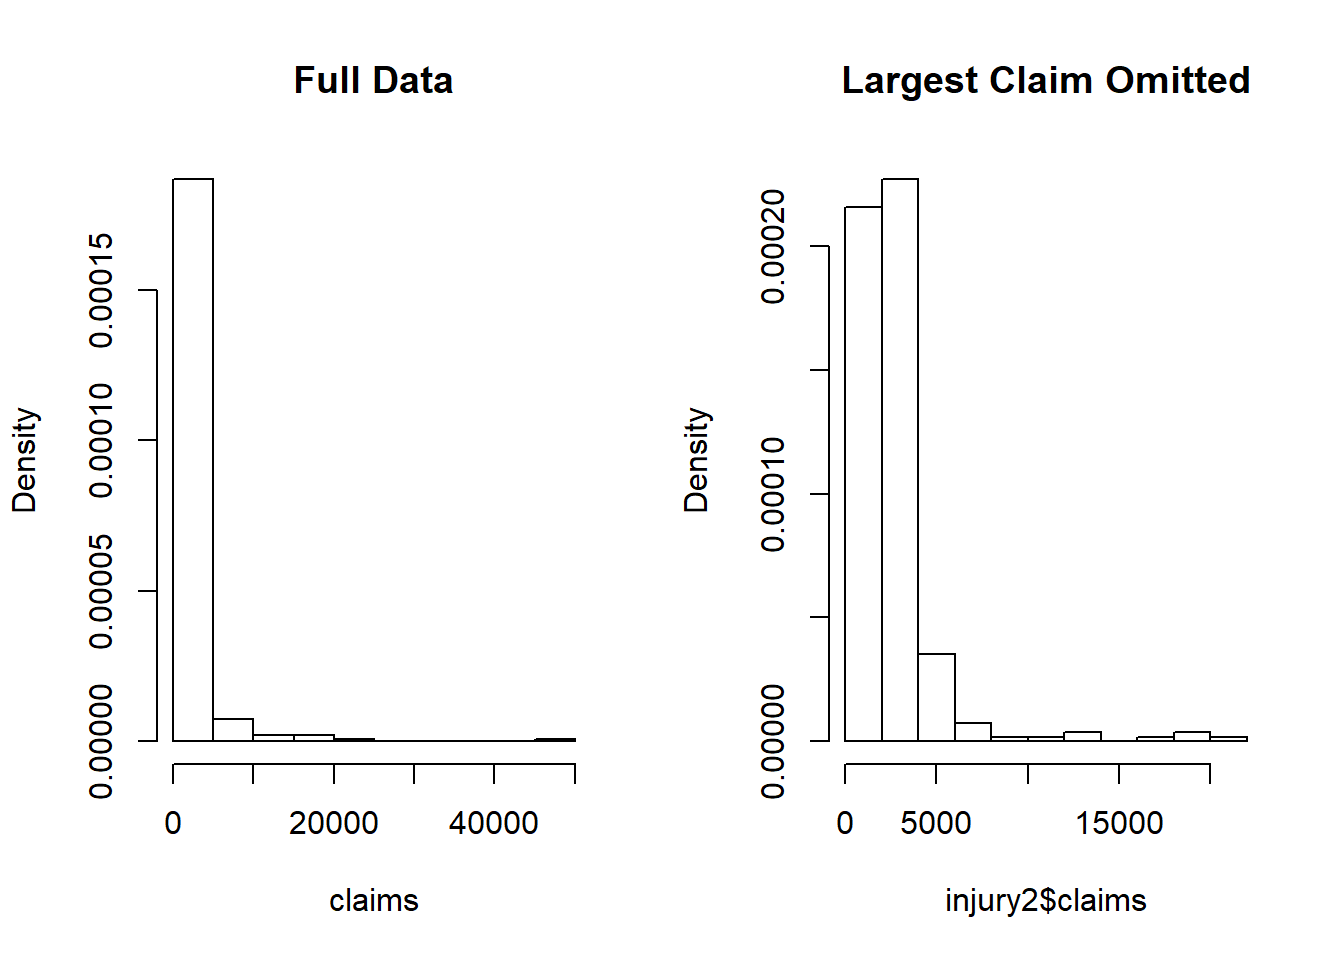
\includegraphics{RegressModelDataCamp_files/figure-latex/unnamed-chunk-32-1.pdf}

\subsection{Exercise. Distribution of transformed bodily injury
claims}\label{exercise.-distribution-of-transformed-bodily-injury-claims}

\textbf{Assignment Text}

We have now examined the distributions of bodily injury claims and its
logarithmic version. Grudgingly, we have concluded that to fit a normal
curve the logarithmic version of claims is a better choice (again, we
really do not like log dollars but you'll get used to it in this
course). But, why logarithmic and not some other transformations?

A partial response to this question will appear in later chapters when
we describe interpretation of regression coefficients. Another partial
response is that the log transform seems to work well with skewed
insurance data sets, as we demonstrate visually in this exercise.

\textbf{Instructions}

Use the code \texttt{par(mfrow\ =\ c(2,\ 2))} so that four graphs appear
in a 2 by 2 matrix format for easy comparisons. Plot the
\href{https://www.rdocumentation.org/packages/stats/versions/3.5.1/topics/density}{density()}
of

\begin{itemize}
\tightlist
\item
  claims
\item
  square root of claims
\item
  logarithmic claims
\item
  negative reciprocal of claims
\end{itemize}

\textbf{Hint}

For negative reciprocal claims, use
\texttt{plot(density(-claims\^{}(-1)))}

\textbf{Pre-exercise code}

\begin{Shaded}
\begin{Highlighting}[]
\CommentTok{# Pre-exercise code}
\NormalTok{injury <-}\StringTok{ }\KeywordTok{read.csv}\NormalTok{(}\StringTok{"CSVData}\CharTok{\textbackslash{}\textbackslash{}}\StringTok{MassBI.csv"}\NormalTok{, }\DataTypeTok{header =} \OtherTok{TRUE}\NormalTok{)}
\CommentTok{#injury <- read.csv("https://assets.datacamp.com/production/repositories/2610/datasets/8cca19d0503fcf6e9d30d9cb912de5ba95ecb9c1/MassBI.csv", header = TRUE)}
\NormalTok{claims <-}\StringTok{ }\NormalTok{injury}\OperatorTok{$}\NormalTok{claims}
\end{Highlighting}
\end{Shaded}

\textbf{SampleCode}

\begin{Shaded}
\begin{Highlighting}[]
\StringTok{`}\DataTypeTok{SampleCode}\StringTok{`}
\CommentTok{#This code helps to organize the four graphs into a 2 by 2 format}
\KeywordTok{par}\NormalTok{(}\DataTypeTok{mfrow =} \KeywordTok{c}\NormalTok{(}\DecValTok{2}\NormalTok{, }\DecValTok{2}\NormalTok{))}
\CommentTok{#Plot the density of claims}
\KeywordTok{plot}\NormalTok{(}\KeywordTok{density}\NormalTok{(___))}

\CommentTok{#Plot the density of square root of claims}
\KeywordTok{plot}\NormalTok{(}\KeywordTok{density}\NormalTok{(___)) }

\CommentTok{#Plot the density of logarithmic claims}
\KeywordTok{plot}\NormalTok{(}\KeywordTok{density}\NormalTok{(___))}

\CommentTok{#Plot the density of the negative reciprocal of claims}
\KeywordTok{plot}\NormalTok{(}\KeywordTok{density}\NormalTok{(___))}
\end{Highlighting}
\end{Shaded}

\textbf{Solution}

\begin{Shaded}
\begin{Highlighting}[]
\CommentTok{# Solution}
\KeywordTok{par}\NormalTok{(}\DataTypeTok{mfrow =} \KeywordTok{c}\NormalTok{(}\DecValTok{2}\NormalTok{, }\DecValTok{2}\NormalTok{))}
\KeywordTok{plot}\NormalTok{(}\KeywordTok{density}\NormalTok{(claims))    }
\KeywordTok{plot}\NormalTok{(}\KeywordTok{density}\NormalTok{(claims}\OperatorTok{^}\NormalTok{(}\FloatTok{0.5}\NormalTok{)))  }
\KeywordTok{plot}\NormalTok{(}\KeywordTok{density}\NormalTok{(}\KeywordTok{log}\NormalTok{(claims)))  }
\KeywordTok{plot}\NormalTok{(}\KeywordTok{density}\NormalTok{(}\OperatorTok{-}\NormalTok{claims}\OperatorTok{^}\NormalTok{(}\OperatorTok{-}\DecValTok{1}\NormalTok{)))  }
\end{Highlighting}
\end{Shaded}

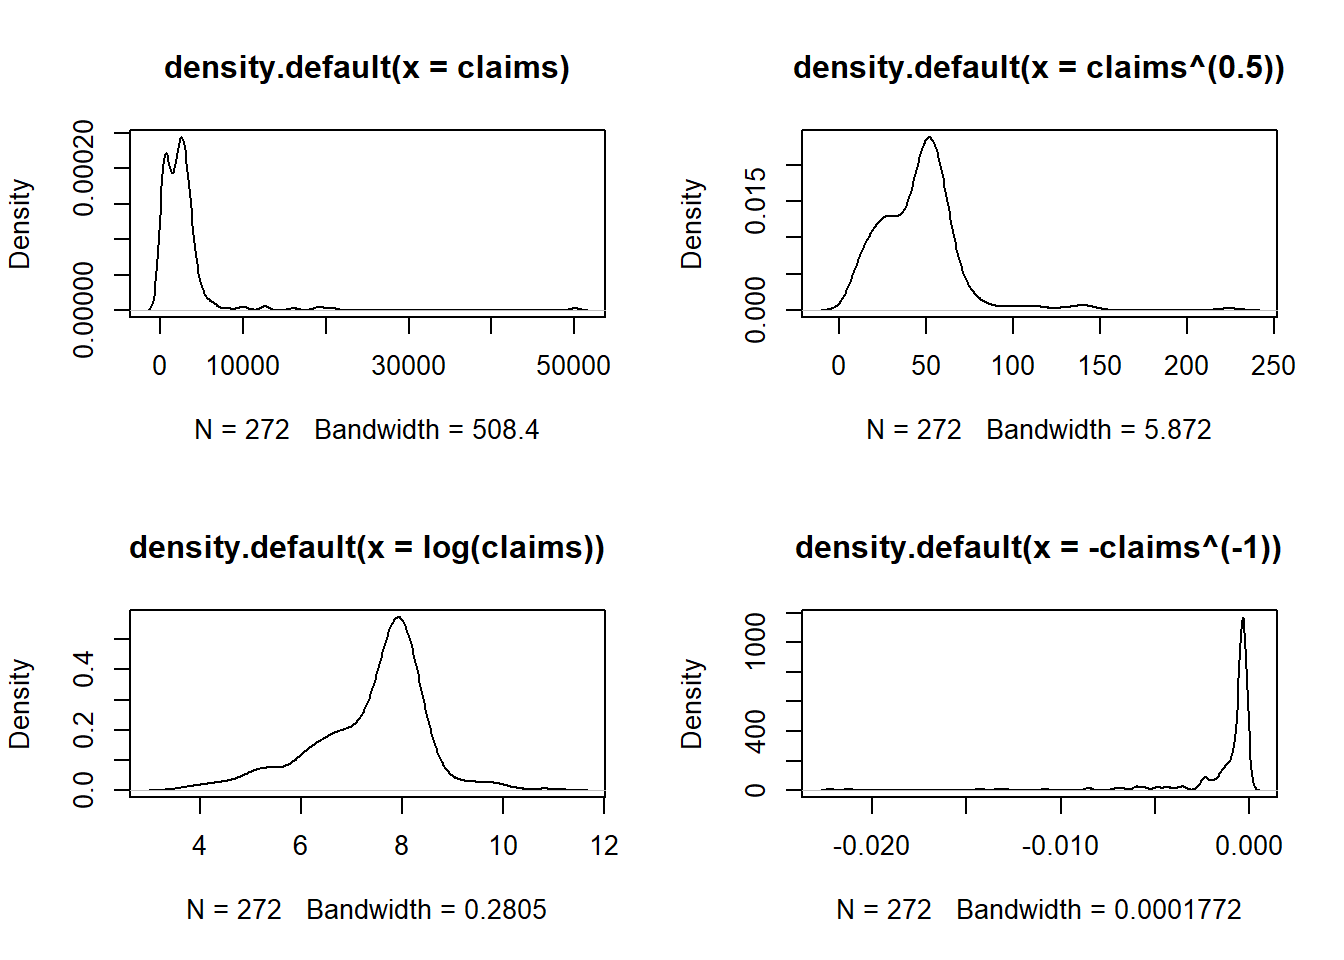
\includegraphics{RegressModelDataCamp_files/figure-latex/unnamed-chunk-35-1.pdf}

\textbf{Submission Correctness Tests (SCT)}

success\_msg(``Excellent! Transformations of data is a tool that
incredibly expands potential applicability of (linear) regression
techniques.'')

\bibliography{Bibliography/LDAReferenceB.bib}


\end{document}
